%=====================================================================
\chapter{Fundamentação teórica}\label{chp}
%========================================================

Como este trabalho propõem a elaboração de um modelo de banco de dados para o LFSR da UERJ, o Capítulo \ref{chp} apresenta conceitos julgados relevantes à metodologia desenvolvida na criação desse projeto piloto. %exemplificar? 



\section{Laboratório de Fotogrametria e Sensoriamento Remoto - LFSR}

O laboratório de Fotogrametria e Sensoriamento Remoto - LFSR faz parte do Departamento de Engenharia Cartográfica - CARTO da Universidade do Estado do Rio de Janeiro - UERJ. Suas instalações são utilizadas para aulas e trabalhos práticos nas disciplinas de Fotogrametria Básica, Fotogrametria Analógica e Analítica, e Aerotriangulação. Uma equipe técnica composta por Professores da UERJ e alunos voluntários e estagiários é responsável pela organização e manutenção de seu espaço físico e seu acervo. O LFSR conta também com o Projeto E-Foto desde Agosto de 2004 em suas instalações, usado como ferramenta auxiliar no aprendizado dos alunos da área.  

\subsection{Instalações do Laboratório de Fotogrametria e Sensoriamento Remoto}

O LFSR se encontra no quarto andar, sala 4044-F, da UERJ. Possui em suas instalações os seguintes equipamentos de fotogrametria, em sua maior parte analógicos: 

\begin{itemize}
    \item Um Aviógrafo Kern PG2 para estéreo compilação fotogramétrica;
    \item Um Aerotriagulador Analógico do tipo Estereoplanígrafo C3;
    \item Quinze Estereoscópios de espelhos;
    \item Centenas de fotogramas em papel e alguns exemplares em diapositivos;
    \item Um Digitalizador Matricial (Scanner) A3Microtek ScanMaker 9800XL;
\end{itemize}

O laboratório também possui computadores (6 desktops e 3 laptops) e algumas poucas licenças de software comercial, priorizando o desenvolvimento e/ou instalação de software livre para a Fotogrametria em seus equipamentos. Seu acervo de dados é composto em sua grande maioria de fotogramas impressos em papel que caracterizam-se de aerolevantamentos passados doados ao Departamento de Cartografia. A figura \ref{lab} representa um demonstrativo dos materiais disponíveis nas instalações do laboratório.

\begin{figure}[!ht]{10cm}
  \caption{Apresentação das instalações e equipamentos do LFSR} \label{lab}
  \centering
  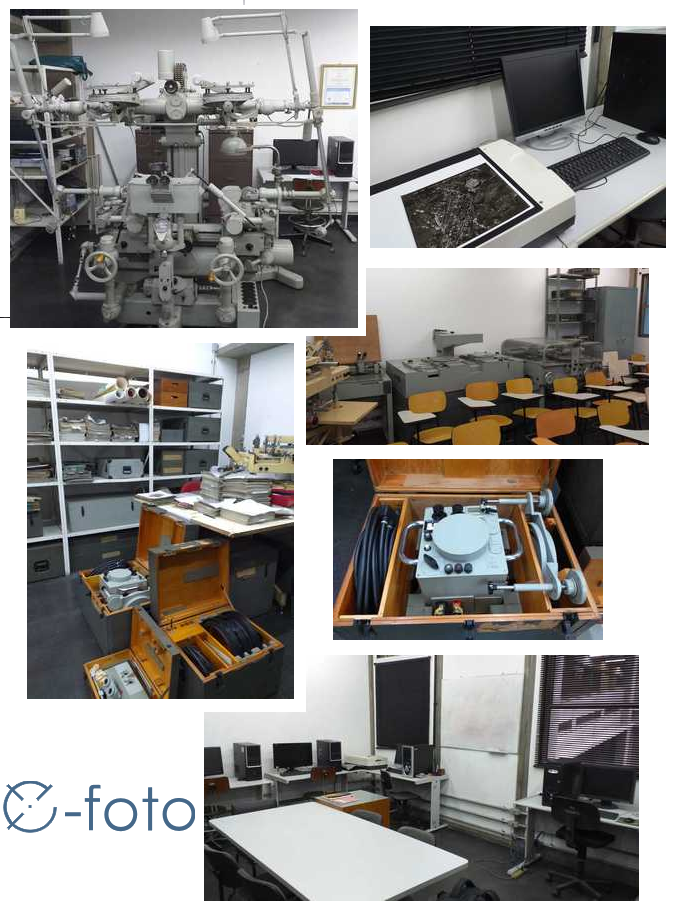
\includegraphics[width=1\textwidth]{figuras/lab.png}
  %\legend{}
  \source{A autora, 2019}
\end{figure}

A ideia da preservação deste acervo, por intermédio da digitalização matricial foi um das motivações para o desenvolvimento deste trabalho. Outro fator motivador foi a necessidade de organizar o acervo, visando não somente ao armazenamento do mesmo mas, principalmente, à sua divulgação e potencial de uso pelos estudantes e professores do Departamento de Engenharia Cartográfica e demais instituições de ensino.

\subsection{Projetos Existentes no Laboratório de Fotogrametria e Sensoriamento Remoto}\label{efoto}

Todo laboratório com fim educacional em geral fornece a infraestrutura necessária para o desenvolvimento de um ou mais projetos que o habilita a exercer sua função acadêmica. O LFSR por sua vez trabalha com o projeto de desenvolvimento do software livre e-foto\footnote{Adota-se a grafia \textit{e-foto} para referir-se ao software e \textit{E-Foto} para referir-se ao seu projeto de desenvolvimento}.

``O projeto E-Foto prevê a implementação de uma solução de uma estação fotogramétrica digital para fins educacionais, de forma livre, habilitando o acesso a tal informação a quaisquer pessoas que o queiram.'' \cite[p. 9]{coelho2007fotogrametria}.

Corroborando com \citeonline{devauxteste}, um `software livre' deve permitir que o usuário: consiga utilizar do programa para quaisquer fins, tenha permissão de redistribuir do programa com a intenção auxiliar outros usuários, a liberdade de aperfeiçoar o software e difundir esses aperfeiçoamentos, e por fim que a plataforma seja de código aberto. Como o projeto E-Foto se enquadra nessas características, além de ser um software com fim educacional, o mesmo atende ``a proposta definida pela Organização das Nações Unidas para a Educação, a Ciência e a Cultura (UNESCO), como um Recurso Educacional Aberto (REA)'' \cite[p.1032]{tramontina69analise}.

De acordo com \citeonline{aguiar2010:desc} o projeto E-Foto conta com vários documentos e dados como tutoriais, trabalhos acadêmicos relacionados ao projeto, o próprio software e etc, em um site próprio com visitas de todo o mundo o que, segundo os autores caracteriza a importância do projeto E-foto como iniciativa no meio acadêmico para a área de Fotogrametria. 

Assim sendo, alunos e pesquisadores da área que usufruem das instalações do LFSR são contemplados com uma plataforma capaz de auxiliar na implementação e ensinamento do processo fotogramétrico. Os resultados de tal uso persistem atualmente sob a forma de arquivos digitais (em formato próprio do software) dos projetos fotogramétricos realizados neste software. Então, a modelagem do banco de dados discutida no capítulo \ref{met} deverá considerar como parte dos requisitos o suporte às informações dos dados dos trabalhos realizados dentro do LFSR. 

Destaca-se também a relevância dos dados de exemplo adotados nos tutoriais publicados no contexto do projeto E-Foto. Por sua importância os mesmos foram selecionados como parte dos dados e documentos que foram usados para a carga inicial e testes do banco de dados desenvolvido nesse trabalho, como será apresentado na seção \ref{carga}.

O processo fotogramétrico possui diversas atividades que podem variar de acordo com o software, porém existem algumas atividades comuns que devem ser destacadas, sendo a maioria identificada facilmente no fluxograma de trabalho da plataforma E-foto, como visto na figura \ref{flux}.

\begin{figure}[!ht]{10cm}
  \caption{Fluxograma de trabalho da plataforma E-foto} \label{flux}
  \centering
  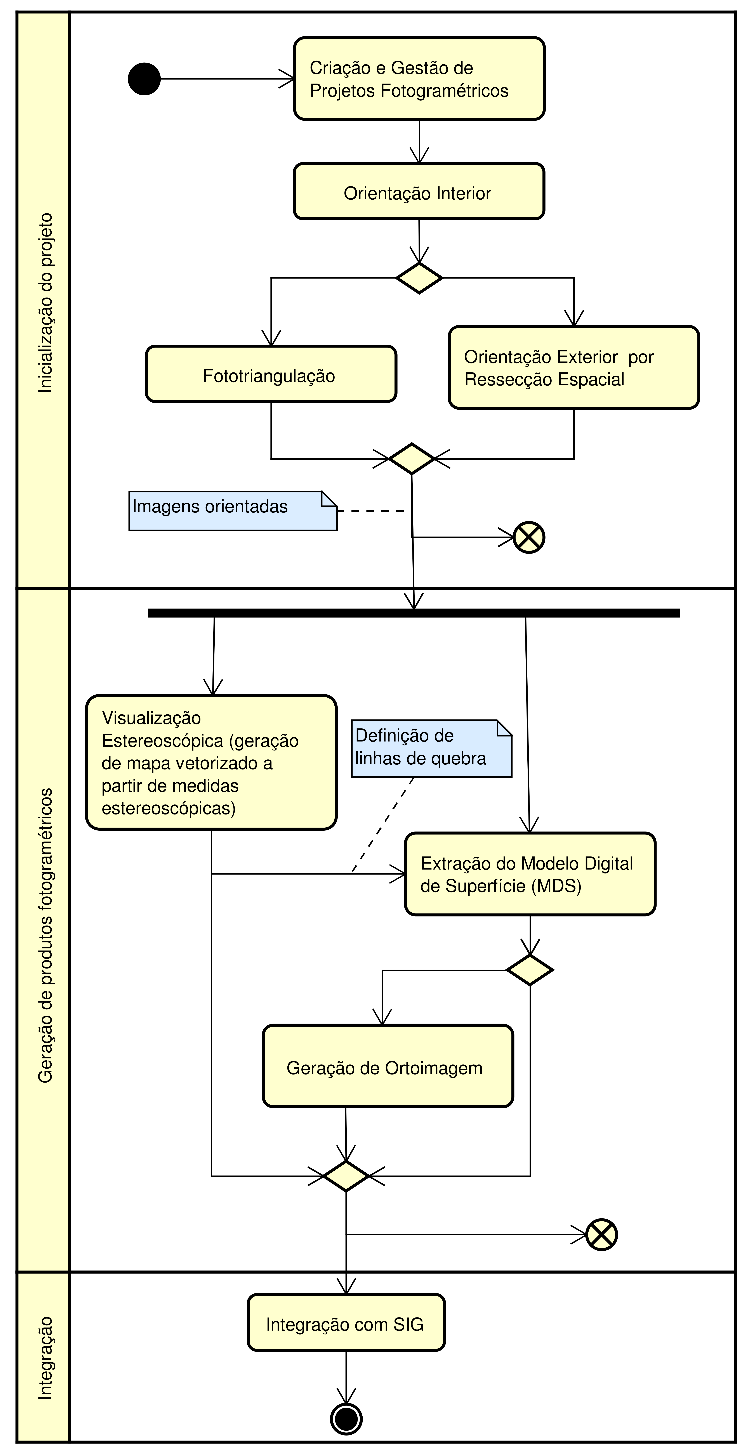
\includegraphics[width=1.2\textwidth, height=1.75\hsize]{figuras/efoto_flux.png}
  %\legend{Texto da legenda quando necessário.}
  \source{\cite{efotoWorkflow}}
\end{figure}

Essas atividades estão distribuídas em 3 fases do projeto. As fases transmitem a compreensão do grau de desenvolvimento do projeto fotogramétrico. Tais fases e atividades são descritas a seguir:

\begin{enumerate}
    \item \textbf{Inicialização do Projeto:} Antes que qualquer produto da fotogrametria possa ser gerado e divulgado para demais processos de produção cartográfica é necessária a realização da aquisição, do cadastro e da orientação (ajustamento) dos dados. Tais atividades são tratadas como fase inicial, pois não produzem produtos finais para processos externos à fotogrametria. As atividades nesta fase são:
    \begin{itemize}
        \item \textbf{Criação e Gerenciamento do Projeto Fotogramétrico:} Nesta atividade do processo o responsável técnico pelo projeto registra os metadados como os obtidos a partir do certificado de calibração e planejamento de voo, que são indispensáveis para os cálculos. No momento inicial de um projeto fotogramétrico ocorrem os levantamentos aéreo e topográfico da região de interesse, resultando na aquisição de dados como as imagens e os pontos de apoio de campo que serão usados no processamento. Esta atividade incluí também o cadastro dos dados adquiridos como resultado dos levantamentos realizados.
        \item \textbf{Orientação Interior:} Nesta atividade do processo as imagens estão sem a referência métrica, tendo suas coordenadas relativas aos \textit{pixels}, isto é, em `linhas' e `colunas'. Logo deve ser feita a reconstrução do feixe perspectivo, um processo que precisa de informações como as coordenada do centro de perspectiva (CP) da câmara e a distância focal. Como resultado são ajustados coeficientes para um modelo paramétrico que relacionam o sistema matricial da imagem com o sistema métrico do sensor por intermédio, por exemplo, da transformação afim\footnote{Apontamentos de aula da disciplina Fotogrametria Analógica e Analítica ministrada pelo Professor Jorge Luís N. e S. Brito}.
        \item \textbf{Orientação Exterior:} A orientação exterior consiste na determinação da posição tridimensional do centro de perspectiva da câmara, em relação ao referencial de coordenadas do terreno, e dos seus respectivos ângulos de atitude, no momento da tomada da fotografia. O cálculo consiste na determinação de seis parâmetros: as coordenadas no espaço-objeto do centro de perspectiva (X0,Y0,Z0) e os ângulos de atitude do sensor ($\phi$,$\omega$,$\kappa$). É importante mencionar que o cálculo dos parâmetros da orientação exterior pode ser realizado para cada imagem isoladamente (atividade de ressecção espacial) ou para o conjunto de imagens que compõem um bloco fotogramétrico, situação na qual o processo adota a atividade de fototriangulação (também conhecida como aerotriangulação).
    \end{itemize}
    \item \textbf{Geração de Produtos:}  Nesta fase são gerados o produtos fotogramétricos propriamente, dentre os quais o projeto E-Foto inclui:
    \begin{itemize}
        \item \textbf{Visualização Estereoscópica:} Permite a observação de modelos estereoscópicos e a restituição fotogramétrica, isto é, a vetorização de superfícies pela obtenção de seus vértices em três dimensões. São produzidas nesta atividade feições vetoriais como pontos, linhas e polígonos.
        \item \textbf{Extração de Modelo Digital de Superfície:} Permite a modelagem da superfície observadas nas imagens do projeto fotogramétrico pela extração automatizada de pontos tridimensionais sobre a superfície. Métodos de interpolação para publicação de modelos regulares são inclusos nesta atividade.
        \item \textbf{Geração de Ortoimagem:} Uma ortoimagem é, por definição, uma imagem que passou pelo processo de ortoretificação e teve os deslocamentos devido ao relevo, removidos nesse processo. Esta atividade se concentra na ortoretificação para imagens isoladas ou blocos. No último caso o produto é chamado de ortomosaico.
    \end{itemize}
    \item \textbf{Integração:} A fase de integração admite que os produtos fotogramétricos sejam disponibilizados nos formatos próprios para uso em demais processos de produção cartográfica. Embora as atividades desta fase possam ser diferenciadas de acordo com o produto fotogramétrico e processo de produção cartográfica, o diagrama simplifica esta fase em uma atividade.
\end{enumerate}

Devido a extensão do fluxo de trabalho, conforme será discutido no capítulo \ref{met}, o escopo da modelagem deverá ser delimitado nas atividades da fase de inicialização do processo fotogramétrico.



\section{Sensoriamento Remoto e Fotogrametria} \label{sensofot}
Sensoriamento Remoto é mais comumente conhecido como uma ciência e técnica que tem por objetivo a captação de informações sobre um objeto, onde não existe contato físico entre o sensor e o objeto de interesse.  Enquanto essa definição não é errada, esta por si só é demasiadamente ampla, o que leva à uma definição mais científica: 

``Sensoriamento Remoto é uma ciência que visa o desenvolvimento da obtenção de imagens da superfície terrestre por meio da detecção e
medição quantitativa das respostas das interações da radiação eletromagnética com os
materiais terrestres.'' \cite[p.3]{meneses2012introduccao}

\subsection{Espectro Eletromagnético}
Os dados obtidos por um processo de sensoriamento remoto dependem da energia com que trabalha o sensor, essa energia é a radiação eletromagnética - REM (ou simplesmente energia eletromagnética), que se propaga no vácuo em forma de senoides, com variações de frequência e comprimento de onda. A figura \ref{wave} ilustra a propagação de uma onda eletromagnética.

\begin{figure}[!ht]{12cm}
  \caption{Representação da propagação de uma onda eletromagnética.} \label{wave}
  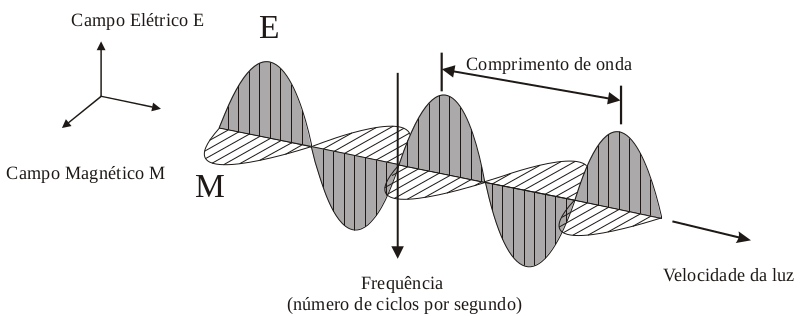
\includegraphics[width=1.1\hsize]{figuras/wave.png}
  %\legend{Texto da legenda quando necessário.}
  \source{\cite{florenzano2007iniciaccao}}
\end{figure}

``Denomina-se espectro eletromagnético as regiões espectrais da REM conhecidas pelo
homem.'' \cite[p.18]{meneses2012introduccao}
De acordo com \citeonline[p.21-24]{moreira2007fundamentos} o espectro eletromagnético possui uma grande variação em seus comprimentos de onda, onde seu comprimento é inversamente proporcional à sua frequência. Isso implica em que nas regiões do espectro onde as ondas são mais curtas, e associadas aos raios cósmicos, a frequência é muito maior do que nas regiões de ondas mais longas, região onde se encontram as ondas longas de rádio frequência.
Essas regiões são apresentadas na figura \ref{espectro}.

\begin{figure}[!ht]{12cm}
  \caption{Ilustração do Espectro Eletromagnético.} \label{espectro}
  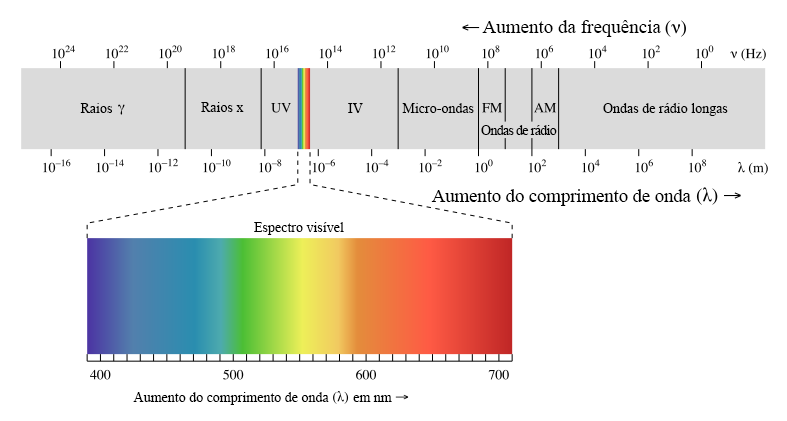
\includegraphics[width=1.1\hsize]{figuras/espectro.png}
  %\legend{Texto da legenda quando necessário.}
  \source{\cite{admirdoresdafisica}}
\end{figure}

Enquanto o olho humano só é capaz de enxergar um intervalo do espectro magnético conhecido como 'luz visível', um sensor remoto é capaz de captar informações espectrais de outros comprimentos de onda de fora desse intervalo. 
\begin{citacao}
    
As imagens [...] devem ser vistas como uma forma de documentos que representam, em escala e sobre um plano 2D, os acidentes e as feições naturais e artificiais da superfície terrestre, a partir da medição de um processo físico da radiação eletromagnética.\cite[p.77]{meneses2012introduccao}
\end{citacao}
Durante anos a fotogrametria foi restrita a imagens fotográficas, somente possíveis pela captação e registro da parte visível do espectro eletromagnético, explicitado na figura \ref{espectro}, porém com os avanços tecnológicos os sensores atuais são capazes registrar informações além desse intervalo, abrindo inúmeras possibilidades para a fotogrametria.  

\subsection{Sensores e Captação de Imagens}\label{sensor_img}
``Os sensores remotos são equipamentos que captam e registram a energia refletida ou emitida pelos elementos da superfície terrestre'' \cite{florenzano2007iniciaccao}.
De acordo com \citeonline[p.9]{lillesand2015remote} a energia de radiação eletromagnética captada por esses sensores deve passar pela atmosfera terrestre.
Contudo, ``a atmosfera interfere na intensidade do fluxo radiante, na distribuição espectral e na direção dos raios incidentes, tanto na sua trajetória
descendente entre o Sol e a Terra como na trajetória ascendente da radiação refletida e
emitida da superfície terrestre para o sensor'' \cite[p.24]{meneses2012introduccao}.

Conforme \citeonline[p.9]{lillesand2015remote}, a energia utilizada pelo sensor remoto ao passar pela atmosfera sofre em seu caminho dois efeitos de distorção: \textit{espalhamento} e \textit{absorção}.

Espalhamento pode ser definido como a dispersão (ou difusão) da radiação eletromagnética por moléculas, ou partículas maiores, presentes na atmosfera. Quando o espalhamento é resultante da presença de moléculas muito menores do que a radiação tem-se o espalhamento \textit{Rayleigh}. Este, resulta normalmente no efeito `nebuloso' na imagem. Quando a partícula possui um tamanho de diâmetro similar ao comprimento da onda o espalhamento resultante é chamado de \textit{Mie}. Esse tipo de espalhamento é geralmente causado por poeira e vapor d'água. Por fim, quando essas partículas são muito maiores do que o comprimento de onda eletromagnético, denomina-se o espalhamento resultante de \textit{Não-Seletivo}. Este é considerado como o pior espalhamento para sensoriamento remoto, pois afeta tamanhos aleatórios de comprimentos de onda de radiação. Um exemplo simples de efeito na imagem é a presença de nuvens na mesma. O índice da presença de nuvens em uma imagem afeta a usabilidade desta em um projeto fotogramétrico e deve ser levada em consideração em momentos como na montagem do bloco de imagens a ser usado num projeto.

Absorção, ao contrário do espalhamento, resulta na perda da radiação. Devido à presença de gases na atmosfera que interagem diretamente com o espectro eletromagnético, a energia é `bloqueada' no caminho entre a fonte de energia e o alvo, ou no retorno, entre o alvo e o sensor remoto. Esta ocorrência gera as chamadas `janelas atmosféricas', que nada mais são do que os intervalos de comprimento de onda não-absorvidos na atmosfera e, portanto, captados pelo sensor.
%VERIFICAR COM NUNES SE ESTE PARÁGRAFO PRECISA SER MODIFICADO OU NÃO!!!!
Corroborando com \citeonline[p.12]{lillesand2015remote},  um sensor não deve ser escolhido arbitrariamente; ao escolhê-lo deve-se levar em consideração os seguintes aspectos:
\begin{itemize}
\item a sensibilidade do sensor;
\item as janelas atmosféricas existentes dentro do comprimento de onda em que se planeja trabalhar;
\item fonte, magnitude e composição espectral da energia de radiação a ser utilizada.
\end{itemize}

Existe um amplo leque de variedade de modelos e fabricantes de sensores remotos. Tendo em vista os efeitos discutidos nos parágrafos anteriores, trata-se agora a da classificação dos sensores.

Segundo \citeonline[p.98]{fitz2008cartografia}, sensores podem ser classificados de acordo com a origem da fonte de energia em  \textit{ativos} e \textit{passivos}.

Sensores ativos são aqueles que possuem fonte de energia interna (ou acoplada ao sensor). Isso significa que a energia necessária para captar a radiação refletida pelo alvo deve ser emitida pelo próprio sensor. O Radar é um bom exemplo desse tipo de sensor, fazendo a captação de dados por meio de ondas de rádio. A figura \ref{sr_ativo} ilustra de forma simplificada um sensor ativo.

\begin{figure}[!ht]{10cm}
  \caption{Ilustração de um sensor ativo} \label{sr_ativo}
  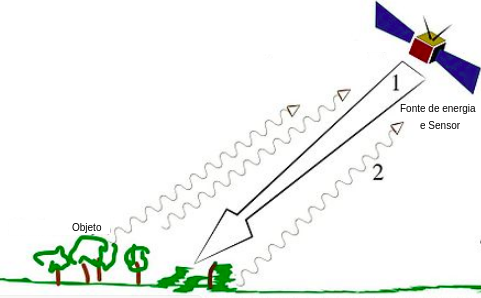
\includegraphics[width=1\hsize]{figuras/sensor_ativo.png}
  \legend{1. A energia é emitida de uma fonte artificial em direção à superfície; 2. A energia é refletida retorna para registro pelo sensor.}
  \source{Adaptação de \cite{sensorfig}}
\end{figure}

Sensores passivos, no entanto, dependem de uma fonte de energia externa e independente do sensor. O Sol é a fonte de energia externa com que trabalha a maioria dos sensores passivos. Neste caso a imagem, gerada precisa ser obtida necessariamente durante o dia. A figura \ref{sr_passivo} ilustra de forma simplificada um sensor passivo.

\begin{figure}[!ht]{10cm}
  \caption{Ilustração de um sensor passivo} \label{sr_passivo}
  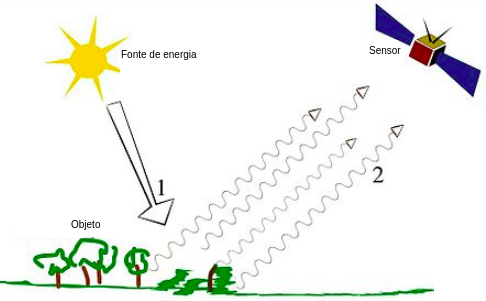
\includegraphics[width=1\hsize]{figuras/sensor_passivo.png}
  \legend{1. A energia é emitida de uma fonte natural e atinge a superfície; 2. A energia é refletida e retorna para registro pelo sensor.}
  \source{Adaptação de \cite{sensorfig}}
\end{figure}

Existem casos, como as câmeras fotográficas digitais, onde o sensor se enquadra em ambas as classificações. Se o `flash' da câmera estiver ativado, a fotografia gerada é proveniente de uma fonte interna, o que caracteriza o sensor como ativo. Porém, se o `flash' estiver apagado, a fotografia vai depender de uma fonte de energia externa, o que define, neste momento, a câmera como um sensor passivo.

De acordo com \citeonline[p.98]{fitz2018geoprocessamento}, outra forma de classificar o sensor é por seu produto. Estes sensores são conhecidos como \textit{imageadores} ou, \textit{não imageadores}. Sensores imageadores, como o próprio nome indica, traduz os dados em formato de imagens. Sensores não imageadores geram, a partir da informações coletadas, dados em formato de tabelas, gráficos e etc. Os dados de sensores não imageadores, geralmente chamados de spectroradiômetros, destinam-se a construir bibliotecas de assinaturas espectrais, que fogem ao escopo deste projeto. Por isso lida-se neste trabalho somente com o sensor imageador.

%falar sobre sensores, como eles funcionam(adicionar ilustração), a diferença entre orbital, comentando brevemente na diferença entre as geometrias de aquisição de imagens, e aéreo e enfatizar a importância do sensoriamento aéreo para o trabalho.
\subsection{Níveis de Aquisição de Imagens}
%nao tenho o texto da florenzano!!!! descobrir a pag!
Segundo \citeonline{florenzano2007iniciaccao} um sensor pode se encontrar em diferentes plataformas sejam elas, terrestres, aéreas ou orbitais.
\citeonline[p.3-4]{meneses2012introduccao} afirma que as fotografias são uma classe de sensores remotos. Isso corrobora a afirmação de que a Fotogrametria é uma forma de Sensoriamento Remoto. Assim sendo, ``convencionou-se usar a classificação de \textit{fotogrametria terrestre}, \textit{fotogrametria aérea} (ou aerofotogrametria) e \textit{fotogrametria orbital} para, grosso modo, expressar esses diferentes modos de posicionar o sensor.'' \cite[p. 18]{coelho2007fotogrametria}

A figura \ref{niveis_sr} ilustra os níveis de plataformas aos quais um sensor pode estar acoplado, o que por sua vez influenciam a distância entre um sensor e o objeto, e o tamanho da área que esse sensor consegue analisar. 

\begin{figure}[!ht]{10cm}
  \caption{Níveis de Plataformas de Coletas de Dados de Sensores.} \label{niveis_sr}
  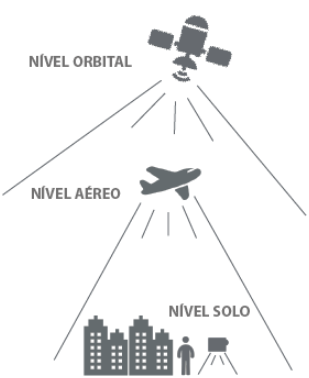
\includegraphics[width=0.5\hsize]{figuras/niveis_sr.png}
  %\legend{Texto da legenda quando necessário.}
  \source{\cite{sensoriamentoremotoweb}}
\end{figure}

Seguindo essa linha de pensamento e utilizando da classificação dada por \citeauthoronline{coelho2007fotogrametria} (\citeyear{coelho2007fotogrametria}, p.18), pode-se dizer que:
\begin{itemize}
    \item \textbf{Fotogrametria Orbital:} se refere a aquisição de imagens que ocorre em nível orbital onde o sensor está acoplado à um satélite. Um satélite por sua vez permanece em órbita durante seu tempo de vida útil transmitindo seus dados a um receptor que se encontra na Terra. Isso permite uma aquisição de imagens abundante onde, dependendo das especificações de seu sensor, podem ter altíssimas precisões muitas vezes necessárias em trabalhos cartográficos. Segundo \citeonline[p. 1]{aquiar2007google}, atualmente imagens de satélites são distribuídos pela internet por plataformas como Google Earth, Microsoft Visual Earth e NASA World Wind. 
    \item \textbf{Fotogrametria Aérea:} também chamada de Aerofotogrametria, acontece quando o sensor se encontra em plataformas de nível aéreo, como aviões e drones. Um exemplo de dados registrados nesse nível são as fotografias aéreas capturadas por câmeras fotográficas métricas. Este assunto será mais explorado posteriormente no item \ref{foto_trad}.
    \item \textbf{Fotogrametria Terrestre:} ou Curta-Distância, se caracteriza essencialmente pelos seus alvos de interesse e a câmara estarem geralmente fixos. A câmara possui seu eixo ótico horizontalizado, o que gera uma imagem horizontal. Essa fotogrametria ocorre no solo, ou a poucos metros acima deste, e investiga objetos geralmente com a intenção de analisar os componentes do mesmo para serviços especializados como a Topografia, a Arquitetura, a Engenharia Civil e etc. Nesses casos a finalidade pode variar de controle de deformação ou desgaste do objeto à restauração do patrimônio histórico de determinada edificação ou o próprio mapeamento topográfico de regiões de difícil acesso.  
\end{itemize}
% falar dos níveis, orbital etc.
Contudo, deve-se ressaltar que o Sensoriamento Remoto, independentemente do nível da plataforma de aquisição em que ocorre, se difere das Fotogrametrias Orbital, Aérea e Terrestre por englobar também sensores não-imageadores (explicados no item \ref{sensor_img}). Ou seja, a fotogrametria tem como foco extração da métrica 3D a partir das imagens 2D. Por outro lado o sensoriamento remoto pode também ter como foco determinar o significado de objetos imageados por interpretação de imagens. 

\subsection{Fotogrametria Aérea Tradicional}\label{foto_trad}
Segundo \cite[p. 16]{coelho2007fotogrametria}, a fotogrametria pode ser definida como ciência e tecnologia capaz reconstruir o espaço tridimensional, ou parte do mesmo (espaço-objeto), a partir das imagens 2D, oriundas da gravação de padrões de ondas eletromagnéticas (espaço-imagem), sem ter nenhum contato físico direto entre sensor e alvo de interesse.

Na Fotogrametria Aérea Tradicional para autores como \citeonline{projeto1999dalmolin}, \citeonline{coelho2007fotogrametria}, entende-se por plataforma um avião ou uma aeronave à qual o sensor está alocado.

Nos dias atuais, os sensores podem ser analógicos ou digitais. O projeto piloto contempla sensores analógicos que obtenham imagens quadro à quadro, em seus certificados de calibração deve estar registrado as informações relativas às marcas fiduciais. Isto se justifica pelo grande número de imagens deste formato existentes no acervo e como será percebido no capítulo \ref{met} o modelo atende a ambos os tipos de sensor, sendo apenas restrito até o momento aos sensores de quadro. Outros tipos de sensores incluem varredores, muito comuns nos satélites.

%FAZER MARCAÇÃO DA PAGINA!!!!
De acordo com \citeonline{wolf2014elements} a Fotogrametria Aérea pode ser subdividida em duas: \textit{Vertical} ou \textit{Oblíqua}. Na vertical o sensor tem seu eixo óptico alinhado verticalmente ao terreno, resultando em uma tomada de foto onde a projeção da imagem produzida fica em paralelo ao plano da região de interesse. A aeronave sofre porém, ao sobrevoar o terreno, leves alterações em seu curso que acarreta numa variação de angulação pequena e não intencional da foto em relação ao plano do terreno gerando assim fotos levemente inclinadas em ângulos geralmente num intervalo de 1$^{\circ}$ a 3$^{\circ}$. Estes são os ângulos de Euler, ou ângulos de atitude, comentados no capítulo \ref{met}. A Oblíqua por sua vez possui uma inclinação intencional onde a mesma pode ser alta a ponto de permitir ser visto a linha do horizonte na fotografia, como ilustrado na figura \ref{obliqua}.

\begin{figure}[!ht]{10cm}
  \caption{Ilustração da angulação e efeito de distorção em imagens geradas por Fotogrametria Aérea Oblíqua} \label{obliqua}
  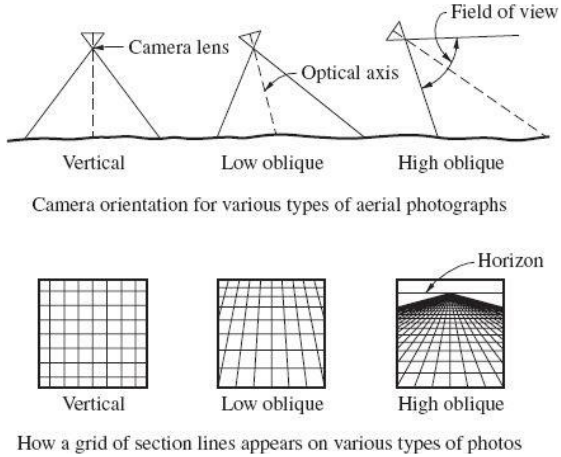
\includegraphics[width=0.75\hsize]{figuras/obliqua.jpg}
  %\legend{Texto da legenda quando necessário.}
  \source{\cite{wolf2014elements}}
\end{figure}

As Fotos geradas pela Fotogrametria Aérea são normalmente destinadas ao mapeamento de uma região de interesse, podendo variar de escalas grandes, comumente usadas em mapas cadastrais, à escalas pequenas, onde o nível de detalhe não precisa ser tão alto para atender o mapeamento escolhido.

Todo projeto fotogramétrico exige diversas considerações a serem tomadas como visto por \citeonline{projeto1999dalmolin} em sua obra. Isto por sua vez acarreta na identificação de dados específicos para a modelagem deste processo. O capítulo \ref{met} apresenta ao longo do modelo todos os dados e particularidades de interesse deste trabalho.

\section{Modelagem de Banco de Dados} \label{mod_bd}

``Dados são fatos em sua forma primária, os quais podem ser armazenados, [...] dados ou fatos organizados de maneira significativa e relacionados formam uma informação'' \cite[p.9]{barcelarbanco}. O que leva à definição: 
%O que é um banco de dados?DEFINIÇÃO
``Um banco de dados é uma coleção de dados relacionados''  \cite[p.3]{navathe2011fundamentals}.

%Qual a importância de um banco de dados?
\citeonline[p.2]{korth2010database} demonstram a importância do banco de dados ao exemplificar sua presença no cotidiano do usuário comum, aquele que não possui grandes conhecimentos computacionais. Esse usuário pode escolher uma música no `\textit{player}' do \textit{smartphone} a caminho do trabalho, verificar sua conta bancária por meio de um site, ao final da manhã e acessar um livro que deseja comprar, no site de uma loja à tarde. Enquanto a interface camufla essas interações, em qualquer um desses exemplos o usuário se encontra em contato direto com um banco de dados. Tendo isso em mente é fácil de entender quando \citeonline[p.6]{taylor2016sql} diz que um banco de dados mais moderno pode armazenar, recuperar e separar dados de forma fácil e rápida, além de armazenar com segurança todos esses dados.

% o que é modelagem de um banco de dados? DEFINIÇÃO
Todavia, antes de existir um banco de dados, o mesmo deve ser idealizado, o que leva a definição de que ``um modelo de dados é um conjunto de conceitos que podem ser usados para descrever a estrutura de um banco de dados'' \cite[p.19]{navathe2011fundamentals}.

\subsection{Sistemas Gerenciadores de Banco de Dados e Extensões Geográficos} \label{sgbdeg}

Segundo \citeonline[p.2-4]{heuser1998projeto} um dos problemas mais comuns na armazenagem de dados é sua redundância, que, por sua vez, se resume a grosso modo como a repetição dos dados armazenados. Essa redundância pode ser controlada, onde a repetição de dados é intencional, ou não controlada, responsável por vários problemas tais como as inconsistências entre os dados armazenados. Para evitar isso é feito um compartilhamento de dados, que atende vários usuários como um conjunto de arquivo integrados, denominado banco de dados. Porém para atender múltiplos usuários o compartilhamento afeta na estrutura do software tornando a estrutura interna dos arquivos mais complexa. A solução para este problema foi a criação de um \textit{Sistema Gerenciador de Banco de Dados}. 
A figura \ref{sgbd} ilustra essa interação entre usuário, SGBD e banco de dados.

\begin{figure}[!ht]{10cm}
  \caption{Ilustração de um sistema de informação baseado em um SGBD} \label{sgbd}
  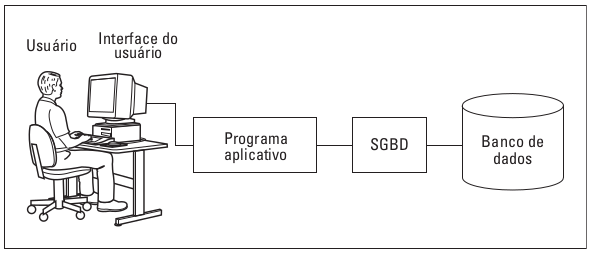
\includegraphics[width=1\hsize]{figuras/esquema_sgbd.png}
  %\legend{Texto da legenda quando necessário.}
  \source{\cite{taylor2016sql}}
\end{figure}
``Um sistema gerenciador de banco de dados (SGBD) é um
sistema de software genérico para manipular bancos de dados'' \cite[p.2]{teorey2014projeto}. Dessa forma, ``o principal objetivo de um SGBD é prover uma forma de armazenar e acessar informações de uma base de dados que seja ambos conveniente e eficiente'' \cite[p.1]{korth2010database}.

``Neste ponto, é importante evitar confundir o BD em si [..] com o programa que o gerenciará, o Sistema Gerenciador de Banco de Dados (SGBD). Em outras palavras, software como Access, MySQL, Oracle, PostgreSQL não são BD, mas sim SGBD'' \cite[p.2]{clickgeogeoprocessamento}.

%arquitetura de banco>DBA>SQL
Alguns autores divergem levemente na arquitetura de um SGBD. Adotando a linha de pensamento de \citeonline[p.12]{barcelarbanco}, a arquitetura de um SGBD pode se dividir em três níveis: \textit{nível externo}, \textit{nível conceitual} e \textit{nível físico}.
Nível externo é o nível em que o usuário `vê' o banco ou partes dele. O acesso do usuário delimita quais dados são visíveis à ele.
Nível conceitual é o nível onde se encontra o modelo conceitual do banco de dados. Neste modelo se define a estrutura de todo o banco, desde conceitos dos dados à como eles se relacionam. A estrutura neste momento é abstrata e não define o local físico de armazenamento. 
Nível físico (ou interno) define o esquema interno, onde é descrito detalhadamente os dados e o caminho de armazenamento dentro do servidor físico. 

Além da arquitetura existem dois conceitos importantes para um banco de dados: \textit{esquema} e \textit{instância}. De acordo com \citeonline[p.8]{korth2010database} em diferentes momentos o banco terá armazenado diferentes dados, estes momentos são chamados de instâncias. A estrutura onde se encontram esses dados é o esquema. Geralmente, enquanto a instância muda constantemente, o esquema raramente sofre mudanças.

Segundo \citeonline[p.22]{navathe2011fundamentals} é essencial para o funcionamento do SGBD uma elaboração cuidadosa do esquema do mesmo. Existe um tipo de dado, chamado \textit{metadado}, armazenado no catálogo do SGBD, também conhecido como dicionário de dados, que descreve as restrições e as construções do esquema, permitindo assim que o SGBD recorra aos metadados quando necessário.   
%[?]O modelo idealizado neste trabalho se encontra no nível conceitual, e o banco de dados resultante foi criado, testado e manuseado no nível externo.

%DBA
Trabalhando no nível conceitual está o administrador do banco de dado, conhecido como DBA. \citeonline[28-29]{korth2010database} afirma que o administrador possui várias funções, dentre elas, criação do banco de dados original, definir a estrutura de armazenamento, realizar modificações nas partes física e conceitual do modelo, garantir ou restringir acesso à outros usuários e o mesmo também é responsável pela manutenção de rotina do SGBD.%PERGUNTAR SE ESTAR CONCEITO ESTÁ CORRETO, POSSO ESTAR ENTENDENDO ERRADO O INGLÊS.

No nível externo se encontra o usuário comum. De acordo com \citeonline[p.12-13]{barcelarbanco} cada um dos usuários possui diferentes \textit{níveis de visão}. O usuário normal não tem visão total do esquema dos dados. O SGBD omite alguns detalhes desnecessários para o usuário de forma que o mesmo tenha um acesso rápido e eficiente aos dados. Essa omissão é feita através de \textit{níveis de abstração}.

\begin{citacao}
    Com o tempo, os SGBD’s passaram a utilizar diferentes formas de representação, ou modelos de dados, para descrever a estrutura das informações contidas em seus bancos de dados. Atualmente, os seguintes modelos de dados são normalmente utilizados pelos SGBD’s: modelo hierárquico, modelo em redes, modelo relacional (amplamente usado) e o modelo orientado a objetos. \cite[p.6]{takai2005intro}
\end{citacao}

Tendo em vista as necessidades deste trabalho, são apresentados os SGBDs baseados no modelo relacional, modelo orientado a objeto e modelo mais recente, modelo objeto-relacional. 

%SGBDR
%\subsubsection{Sistema Gerenciador de Banco de Dados Relacional}\label{sgbdr}
\subsubsection{Modelos de SGBDs}\label{sgbdr}

\begin{citacao}
    ``A abordagem relacional aos dados está baseada na observação de que arquivos que obedecem a certas limitações podem ser considerados como relações matemáticas, e consequentemente a teoria elementar de relações pode ser usada para lidar com vários problemas práticos dos dados desses arquivos'' \cite[p.77]{date1989introducao}.
\end{citacao}

Isso significa que ``o modelo relacional implementa estruturas de dados organizadas em relações'' \cite[p.8]{takai2005intro}. 
Porém antes de se se entender melhor essas `relações' deve-se mencionar que existe uma questão de inconsistência para a terminologia usada na literatura para o banco de dados. Isso se deve pelo seguinte motivo:

``A principal linguagem de manipulação de dados em sistemas de bancos de dados relacionais é o SQL'' \cite[p.9]{alexandruk2011modelagem}. Devido ao desenvolvimento e expansões ao longos dos anos o SQL foi `adaptado' e padronizado tanto pela ANSI quanto pela ISO, tornando a linguagem como padrão para banco de dados tanto relacionais quanto de outros tipos. Isso gera uma `confusão' dentre muitos usuários de banco de dados, principalmente relacionais, portanto deve-se ressaltar que ''SQL e o Modelo Relacional não são a mesma coisa'' \cite{date2011sql}.

A citação, a seguir, explica a estrutura de um banco de dados relacional e exemplifica a questão discutida acima sobre terminologia:
\begin{citacao}
    A estrutura fundamental do modelo relacional é a relação (tabela). Uma relação é constituída por um ou mais atributos (campos) que traduzem o tipo de dados a armazenar. Cada instância do esquema (linha) é chamada de tupla (registro) \cite[p.8]{takai2005intro}.
\end{citacao}


Percebe-se que o autor ao explicar as definições de `relação', `atributo', `instância de esquema' e `tupla' usa dois termos para cada definição. Enquanto exite terminologias mais comuns na literatura, cada autor usa em seus textos a de sua preferência. 

Para facilitar a compreensão deste trabalho, não se adotará uma terminologia específica, de forma que todo e qualquer termo utilizado será previamente ou posteriormente explicado. 

Voltando à explicação dada por \citeauthor{takai2005intro} acima, a figura \ref{tabelas_exe} ilustra um exemplo de dados em um SGBDR.  

\begin{figure}[!ht]{10cm}
  \caption{Exemplos de tabelas que podem ser armazenadas em um SGBDR} \label{tabelas_exe}
  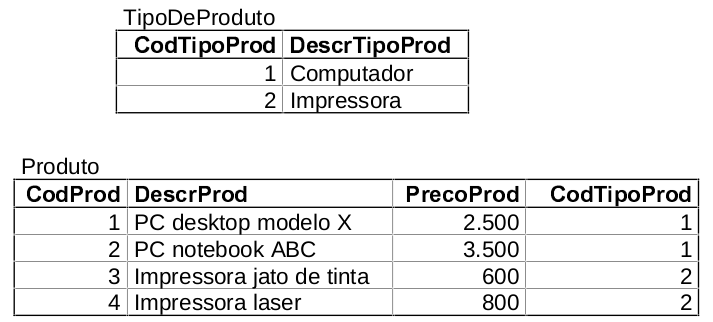
\includegraphics[width=1\hsize]{figuras/tabelas_exemplo.png}
  %\legend{Texto da legenda quando necessário.}
  \source{\cite{heuser1998projeto}}
\end{figure}

Na figura \ref{tabelas_exe} existem duas tabelas chamadas de `TipoDeProduto' e `Produto'. Na primeira tabela encontra-se dois atributos `CodTipoProd' e `DescrTipoProd' enquanto na segunda tabela tem-se `CodProd', `DescrProd', `PrecoProd' e `CodTipoProd' como atributos. Analisando ainda a figura \ref{tabelas_exe} percebe-se um padrão para cada atributo. Esse padrão é denominado \textit{domínio}. Pode-se supor que o domínio do atributo `CodProd' é do tipo `INT', o que significa que naquela tabela serão somente armazenados valores de números inteiros. Porém no atributo `DescrProd' o domínio pode ser do tipo `VARCHAR', que aceita valores textuais ou numéricos como texto com variação de 1 a 8000 bytes. Os tipos de domínios serão explorados mais a frente.

Contudo, existem dados mais complexos, como por exemplo geometrias localizadas no espaço geográfico, que o SGBDR não comporta. Para esses dados foi adotado outro método de modelagem, que utiliza não só os recursos básicos relacionais como também o SQL provido das extensões orientadas a objetos para suporte espacial necessárias. O SGBD de interesse para o trabalho será discutido no próximo item.

%\subsubsection{Sistema Gerenciador de Banco de Dados de Objetos} %PEDIR AO IRVING PARA CHECAR ESTE ITEM, ACHO QUE ESTA FALTANDO MENCIONAR ALGUMA COISA, OU DAR UMA EXPLICAÇÃO QUE ME PERMITA USAR UM TERMO ESPECÍFICO...
%Definição de um SGBDO
\citeonline[p.145]{teorey2014projeto} comenta que a modelagem orientada a objetos é uma forma de mapear o mundo real. 
\begin{citacao}
    A motivação para seu surgimento está em função dos limites de armazenamento e representação semântica impostas no modelo relacional. Alguns exemplos são os sistemas de informações geográficas (SIG)[..] O termo Modelo Orientado a Objetos é usado para documentar o padrão que contém a descrição geral das facilidades de um conjunto de linguagens de programação orientadas a objetos e a biblioteca de classes que pode formar a base para o Sistema de Banco de Dados. \cite[p.8-9]{alexandruk2011modelagem}
\end{citacao}

Em outras palavras, ``com tipos de sistemas complexos pode-se representar conceitos de modelos ER. Como atributos compostos, atributos multi-valorados, generalização, e especialização diretamente, sem a tradução complexa do modelo relacional'' \cite[p.947]{korth2010database}

``Um recurso dos bancos de dados de objeto é o poder que eles dão ao projetista para especificar tanto a \textit{estrutura} dos objetos complexos quanto as \textit{operações} que podem ser aplicadas a esses objetos'' \cite[p.236]{navathe2011fundamentals} 

Pensando na estrutura, segundo \citeonline[p.4]{alexandruk2011modelagem} o pensamento por trás da orientação a objeto em banco de dados consiste na concepção de herança entre os dados. Estes são tratados como dados abstratos, e portanto objetos. Na abstração ``a ideia básica é retirar os detalhes e reter exatamente o máximo da complexidade da vida real quanto for exigido para a tarefa em mãos'' \cite[p.142]{teorey2014projeto}.  Assim os dados podem ser agrupados como um único objeto, estruturando-os em classes e superclasses. Observa-se assim hierarquias, como demonstrado na figura \ref{heranca_obj}.

\begin{figure}[!ht]{10cm}
  \caption{Exemplo de herança na orientação objeto.} \label{heranca_obj}
  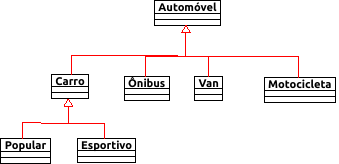
\includegraphics[width=1\hsize]{figuras/heranca.png}
  %\legend{Texto da legenda quando necessário.}
  \source{A autora}
\end{figure}

Analisando a figura \ref{heranca_obj} tem-se uma superclasse `Automóvel', que se subdivide em várias classes. Das classes `Carro', `Ônibus',`Van' e `Motocicleta', qualquer dado da classe `Carro' pode ser entendida como do tipo subclasse `Popular' ou `Esportivo'.  De forma simples, isso significa que na herança, para cada entrada de dado, existirá atributos em comum dentre os objetos dessa herança. Todo registro na entidade `Popular' terá também dados complementares relacionados a esse registro transcritos no objeto `Carro' e, num nível acima, no objeto `Automóvel'. 

Esse tipo de distinção entre os dados como objeto não seria possível em um banco de dados relacional, pois de acordo com \citeonline[p.4]{alexandruk2011modelagem}, as relações de um banco só possuíam valores atômicos até então.
Se `Automóvel', da figura \ref{heranca_obj}, fosse aplicado em um banco de dados relacional, esta superclasse seria uma tabela com dúzias de atributos com muitos deles possuindo dados repetidos para poder simplesmente armazenar um tupla. Isso afeta a eficiência com a qual o banco acessa os dados dessa tabela.

Como este trabalho é voltado para, entre outros, dados geográficos, no item \ref{ext_geo} será comentado superficialmente sobre extensões geográficas que são aceitas como padrão\footnote{Seguindo a especificação OpenGIS\cite{opengis}} para os SGBDs que implementem esses tipos de dados complexos. 


%qual a diferença entre um SGBDR e um SGBDO?

%\subsubsection{Sistema Gerenciador de Banco de Dados Objeto Relacional}
%SGBDOR (não preciso entrar a fundo nisso, pois ao explicar SGBDR e SGBO eu ja mato o assunto)

Segundo \citeonline[p.15-18]{navathe2011fundamentals} dados complexos, como os dados geográficos não são atendidos pelo banco de dados relacional devido às suas características. Porém os mesmos, como comentado anteriormente, podem ser modelados de acordo com a estrutura de um banco de dados orientado a objeto. 

Assim sendo, devido a sua simplicidade, existe uma preferência ao SGBDR no mercado em comparação ao SGBDO, ``muitos conceitos orientados a objeto foram incorporados nas versões mais recentes do SGBD relacional, levando a sistemas de gerenciamento de banco de dados objeto-relacional, conhecidos como SGBDORs'' \cite[p.16]{navathe2011fundamentals}.
\begin{citacao}
    Esses sistemas [...] implementam uma camada de abstração de dados em cima de métodos relacionais, o que torna possível a manipulação de dados mais complexos. [...] Todas as características relacionais permanecem, ou seja, as tabelas continuam a existir, porém elas possuem alguns recursos adicionais.\cite[p.4]{alexandruk2011modelagem}.
\end{citacao}

\subsubsection{Extensões Geográficas}\label{ext_geo}
%Qual o diferencial da informação geográfica? 
``Modelos de dados para aplicações geográficas têm necessidades adicionais, tanto com relação à abstração de conceitos e entidades, quanto ao tipo de entidades representáveis e seu inter-relacionamento'' \cite[p.86]{borges2005modelagem}. Em outras palavras,``a modelagem de dados geográficos é uma atividade complexa porque envolve a discretização do espaço como parte do processo de abstração, visando obter representações adequadas aos fenômenos geográficos'' \cite[p.30]{queiroz2006tutorial}.


De acordo com \citeonline[p.358-359]{guting1994an} bancos de dados espaciais proveem a tecnologia básica para aplicações como Sistemas de Informação Geográficos - SIG (em inglês Geographic Information System - GIS). Eles devem três características básicas. 
\begin{itemize}
    \item Bancos de dados espaciais devem ser também bancos de dados, pois todo dado espacial se relaciona de alguma forma com dados alfanuméricos. Isso implica no banco ter capacidade de lidar com esse tipo de dado além do espacial.
    \item Deve oferecer tipos específicos de `data type' que atendam as características espaciais no modelo de dados e na linguagem de consulta. Esse `data type' determina o domínio do atributo, assim permitindo que o banco trabalhe com os dados geométricos relacionados ao terreno, da mesma forma que suas relações.
    \item Fornecer indexação espacial e algoritmos voltados para o tratamento desses dados, de forma que o sistema seja capaz de obter uma coleção de objetos de um conjunto de dados presentes num terreno. Eles devem também ser capaz de conectar objetos de diferentes classes por seus dados espaciais.
\end{itemize}

``No que se refere ao ramo de banco de dados (BD) com extensões geográficas os nomes mais citados em debates em geral são Oracle Spatial, PostgreSQL/PostGIS e MySQL Spatial'' \cite[P.1]{clickgeosgbd}

\subsection{Processo de Desenvolvimento de Sistemas} \label{proc}

\begin{citacao}
Método é um procedimento ou técnica utilizado para obter um determinado resultado. Também pode ser definido como uma forma de agir em uma determinada situação a fim de regularizar uma tarefa. Com essa definição é possível entender o porquê é fácil encontrar várias metodologias para o desenvolvimento de documentação de software. Isso acontece porque são vários os tipos de software que são desenvolvidos em várias linguagens para diversos ambientes e desenvolvidos em diversos modelos de sistemas de informação, tais como baseado em fluxo de dados, relacionais e orientado a objetos. \cite[p.402]{keila2010metodologias}
 \end{citacao}
 
De acordo com \citeonline[p.2-3]{dos2004comparaccao} existem metodologias tradicionais e metodologias ágeis. Pode-se entender como modelo sequencial, que é um modelo tradicional,  aquele onde cada etapa deve ser finalizada antes de outra ser iniciada, ou seja, deve seguir uma sequência, apresentado inicialmente no modelo de Royce. O modelo de cascata, como ilustrado na figura \ref{waterfall}, é um exemplo de modelo sequencial.

\begin{figure}[!ht]{10cm}
  \caption{Ilustração do modelo em cascata.} \label{waterfall}
  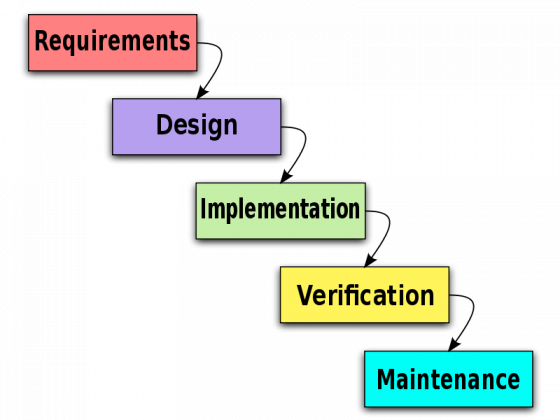
\includegraphics[width=0.6\hsize]{figuras/Waterfall-Model-560x420.png}
  \source{\cite{tech2019waterfall}}
\end{figure}

Onde os termos `Requirements', `Design', `Implementation', `Verification' e `Maintenance' podem ser entendidos de forma geral como as etapas de um processo de desenvolvimento de sistemas. Assim se referem respectivamente a: a definição de requisitos, projeto do software, implementação e teste unitário, integração e teste do sistema, operação e manutenção. 
Segundo \citeonline[p.2]{tech2019waterfall} um modelo monolítico, como o apresentado, possui uma grande desvantagem: pouca, se não inexistente, maleabilidade que comporte mudanças ocorridas ao longo do processo. Desta forma, \citeonline[p.4]{badolato2019} afirma que se houver necessidade de mudanças durante o processo com este modelo, todo o trabalho realizado até aquele ponto é perdido. Em suma, a expectativa de reaproveitar o trabalho nos leva à reflexão de como adaptar o modelo para ser capaz de lidar com mudanças.

Uma forma de se resolver este problema foi a integração de componentes, ilustrada na figura \ref{integracao}. Desta forma o processo é subdividido em partes com cada parte sendo trabalhada individualmente. Assim acarretando numa retro-alimentação, também conhecida como incremental. Este modelo de processo continua sendo monolítico, porém agora existe uma maior maleabilidade ao longo do desenvolvimento.

\begin{figure}[!ht]{15cm}
  \caption{Modelo de processo incremental.} \label{integracao}
  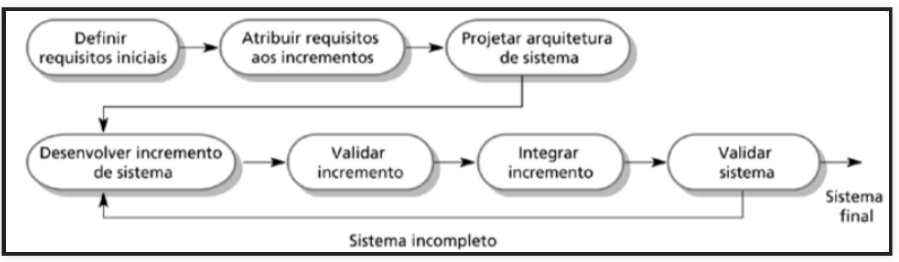
\includegraphics[width=1\hsize]{figuras/integracao.png}
  %\legend{Texto da legenda quando necessário.}
  \source{\apud{sommerville2008engenharia}{badolato2019}}
\end{figure}

Neste caso, os requisitos iniciais são identificados, atribuídos aos incrementos, como uma lista de atividades, e geram então uma visão macro da arquitetura do projeto. A partir daí cada incremento é trabalhado separadamente, enquanto ocorre a retro-alimentação e consequente revisita das atividades do processo. Segundo ainda \citeonline{badolato2019} a alteração pela simples adição de retroalimentação no processo modelado na figura \ref{waterfall}, enquanto trata das mudanças, não apresenta solução para o problema do tempo gasto quando os projetos são demasiadamente grandes, o que incide no atraso da entrega do sistema em face ao prazo. 

O atraso na entrega do sistema pode gerar `tensão' entre o implementador e o cliente. Visando solucionar este problema, a abordagem se torna ``em espiral'', na qual o produto é quebrado em pequenos componentes, que são incorporados ao produto e entregues ao cliente a medida que são finalizados. Esta abordagem enquanto mais rápida pode ser também rígida e complexa.

Tomando por base o modelo em espiral, existe ainda a necessidade de uma padronização do processo de desenvolvimento de software, onde a interação é dinâmica, fato que levou ao modelo denominado ``ágil''.

\begin{citacao}
O termo “Metodologias Ágeis” tornou-se popular em 2001 quando dezessete especialistas em processos de desenvolvimento de software representando os métodos Scrum [Schwaber e Beedle (2002)], Extreme Programming (XP) [Beck (1999)] e outros, estabeleceram princípios comuns compartilhados por todos esses métodos.\cite[p.3]{dos2004comparaccao}
\end{citacao}

O modelo ágil, diferentemente do tradicional, é cíclico. Isso permite que os requisitos estabelecidos inicialmente sejam modificados de acordo com a evolução do desenvolvimento do sistema. A implementação também faz parte de cada ciclo, diferentemente do modelo monolítico onde antes a implementação só ocorria em um momento avançado do desenvolvimento. A tabela \ref{agil_trad} exibe as principais diferenças entre o modelo tradicional (monolítico) e o modelo ágil (cíclico).

\begin{table}[!ht]{14cm}
  \caption{Comparação entre modelo Ágil e Modelo Tradicional.}\label{agil_trad}
    \begin{tabular}{cc}
    \hline
    \rowcolor[HTML]{333333} 
    {\color[HTML]{FFFFFF} \textbf{Modelo Ágil}} & {\color[HTML]{FFFFFF} \textbf{Modelo Tradicional}} \\ \hline
    \rowcolor[HTML]{EFEFEF} 
    \begin{tabular}[c]{@{}c@{}}Abordagem iterativa, permitindo que \\ ocorram mudanças durante todo o \\ processo\end{tabular} & \begin{tabular}[c]{@{}c@{}}Abordagem sequencial, cada, etapa é \\ fechada e precisa ser finalizada antes \\ do inicio na etapa seguinte\end{tabular} \\
    \begin{tabular}[c]{@{}c@{}}Funciona bem quando o projeto não \\ é conhecido\end{tabular} & \begin{tabular}[c]{@{}c@{}}Atende melhor quando se sabe o \\ projeto\end{tabular} \\
    \rowcolor[HTML]{EFEFEF} 
    \begin{tabular}[c]{@{}c@{}}É importante ter acesso ao cliente \\ durante todo o processo\end{tabular} & \begin{tabular}[c]{@{}c@{}}O cliente só é consultado no início e \\ posteriormente na entrega do software\end{tabular} \\
    \begin{tabular}[c]{@{}c@{}}Permite verificações e validações \\ preliminares, aumentando as chances \\ de sucesso no programa final\end{tabular} & \begin{tabular}[c]{@{}c@{}}Não permite validações ou verificações \\ durante, processo, diminuindo as \\ chances de sucesso ao final do processo\end{tabular} \\
    \rowcolor[HTML]{EFEFEF} 
    \begin{tabular}[c]{@{}c@{}}Software é exaustivamente testado \\ durante todo o processo\end{tabular} & \begin{tabular}[c]{@{}c@{}}Teste só pode ser realizado ao final do \\ processo\end{tabular} \\
    \begin{tabular}[c]{@{}c@{}}O implementador tem total flexibilidade \\ dentro dos parâmetros do programa\end{tabular} & \begin{tabular}[c]{@{}c@{}}O implementador fica preso a \\ documentação inicial e tem pouca \\ flexibilidade no desenvolvimento \\ do sistema\end{tabular} \\ \hline
    \end{tabular}
  \source{A autora.}
\end{table}


Existem muitas práticas usadas na atualidade em conjunto com os modelos ágeis para desenvolvimento de um sistema.

Um exemplo de prática Ágil é o Test Driven Development (TDD). De forma resumida pode-se dizer que o TDD consiste no teste e erro. Num primeiro momento o desenvolvedor escreve o suficiente do código para testa-lo. Em seguida realiza esse teste com a expectativa de falhar (1) para evidenciar que o teste é suficientemente crítico. Em seguida o código deve ser consertado a ponto de passar no teste já estabelecido (2). Posteriormente o código deve sofrer alterações e incrementos de forma a ser melhorado (3). Ao final dessa etapa o código deve ser novamente testado com a perspectiva de falhar, logo voltando a etapa inicial para ser capaz de tratar limites, exceções ou novos problemas não abordados nas iterações iniciais. A imagem \ref{TDD} ilustra o fluxograma de um TDD.

\begin{figure}[!ht]{10cm}
  \caption{Fluxograma do TDD.} \label{TDD}
  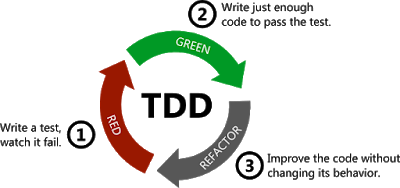
\includegraphics[width=0.75\hsize]{figuras/tdd_flow.png}
  %\legend{Texto da legenda quando necessário.}
  \source{\cite{chairat2017}}
\end{figure}

``A pequena granularidade do ciclo test-then-code dá um feedback contínuo ao programador. Falhas são identificadas mais rapidamente, enquanto o novo código é
adicionado ao sistema. Assim, o tempo de depuração diminui compensado pelo tempo de escrita e execução dos casos de teste'' \cite[p.4]{borges2006conceitos}

Um problema comum neste método é a forma de raciocinar do implementador. Utilizando esta prática ágil não se começa com um código completo, mas sim com um pequeno pedaço dele, que a partir destes testes cresce até atingir os objetivos estabelecidos pelo desenvolvedor. 

O RUP (Rational Unified Process), que é um exemplo de processo moderno baseado na UML e será apresentado posteriormente no item \ref{itemmodl}, foi criado pela mesmo grupo responsável pela criação da UML. Enquanto o modelo não é usado diretamente no trabalho, ele expõem conceitos relacionados à evolução da apresentado pelas metodologias ágeis. A figura \ref{RUP} apresenta o modelo RUP.

\begin{figure}[!ht]{10cm}
  \caption{RUP - Rational Unified Process.} \label{RUP}
  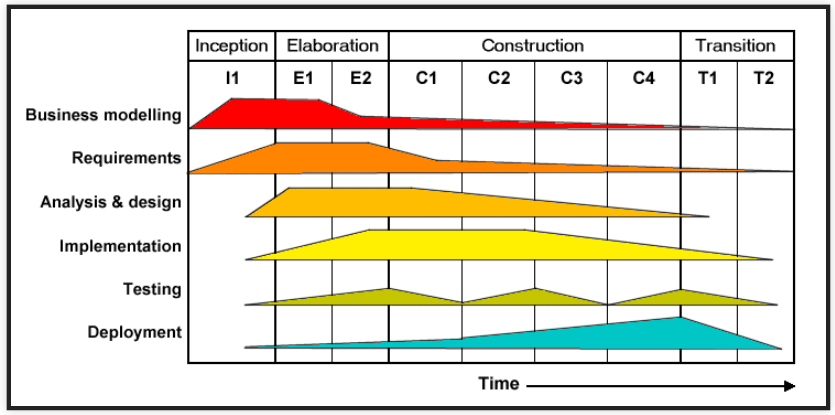
\includegraphics[width=1\hsize]{figuras/rup.png}
  %\legend{Texto da legenda quando necessário.}
  \source{\apud{RUP}{badolato2019b}}
\end{figure}

Analisando a figura \ref{RUP} percebe-se uma distribuição do esforço no desenvolvimento das atividades de cada uma das fases do processo. A um primeiro momento se tem maior esforço atribuído às atividades de definição das regras do negócio e o levantamento dos requisitos, mais a frente durante a fase de elaboração o foco leva a um maior esforço para análise e projeto, durante a construção percebe-se uma carga maior para as atividades de elaboração e teste, sendo que este último está presente durante todo o processo, tendo `picos' ao final de marcos nos quais novos componentes foram construídos e precisam ser aprovados para viabilizar sua entrega. Por último tem-se a aplicação/entrega do sistema que cresce a medida em que as fases finais do processo se aproximam.



\subsection{Conceito de Requisitos de Sistemas} \label{conceitos_requisitos}
Segundo \citeonline[p.3-5]{teorey2014projeto} o primeiro procedimento na elaboração de um banco de dados é a \textit{análise de requisitos}. Parte fundamental do esquema conceitual, os requisitos são especificados a partir de encontros entre o desenvolvedor do banco de dados e o cliente. As informações colhidas dessa reunião geram os requisitos que servirão para restringir e modelar o banco no nível abstrato. Sabendo que ``o esquema conceitual tem como objetivo servir como uma fundação sólida e duradora para a operação global da empresa'' \cite[p.425]{date2011sql}, fica fácil entender que os requisitos são fundamentais para todo o processo de desenvolvimento do sistema.  

De acordo com \citeonline[p.3]{badolato2019b} a primeira coisa a ser feita é o \textit{estudo de viabilidade}.
O estudo de viabilidade pode ser considerado uma etapa 'pré-projeto', onde se pesquisa quais são os possíveis problemas a serem encontrados durante a realização do processo e quais possíveis formas de solucionar esses problemas. Logo em seguida vem a etapa de \textit{elicitação e análise}.

A elicitação e análise de requisitos, é um detalhamento do projeto que ocorre assim que o mesmo é iniciado. Segundo \citeonline[p.14-20]{souza2014banco}, o problema é identificado por meio de perguntas simples, assim estabelecendo: 
\begin{itemize}
    \item uma ideia básica do problema;
    \item quem é afetado de fato por esse problema;
    \item qual é ideia geral por trás da solução planejada;
    \item uma comunicação eficiente entre o produtor e o cliente.
\end{itemize}
Obviamente as perguntas iniciais definem o problema em escopo geral. Segundo esse mesmo autor, para elicitar os requisitos, logo identificar o problema, existem várias técnicas. Dentre elas: amostragem, investigação, entrevista, observação, elaboração de questionários, prototipação etc. 
Neste trabalho a elicitação dos requisitos foi realizada por meio de \textit{brainstorm}.

\textit{Brainstorming} é uma
\begin{citacao}
 ferramenta para geração de novas ideias sobre um determinado assunto. A técnica deve ser livre de críticas que inibam a contribuição dos participantes. O foco é a geração de ideias que podem estar relacionadas às causas, modos de abordagem ou ações a serem tomadas sobre determinado assunto.\cite[p.7]{subplan2014}
\end{citacao}

De acordo com \citeonline[p.109]{leffingwell2000managing}, \textit{brainstorm} possui dois objetivos, a geração e redução de ideias. Primeiro ocorre a exposição de ideias pelos participantes da \textit{brainstorm} e depois essas ideias são reduzidas por meio de organização, catalogação, expurgo de duplicatas etc.

No levantamento de requisitos isso implica em uma ou mais reuniões entre produtor e cliente onde o problema é apresentado pelo cliente. O produtor então pergunta sobre esse problema e expõem possíveis soluções para o mesmo. Durante uma \textit{brainstorm} o problema e as soluções são escritas em um local qualquer, desde um quadro a folhas de papel, assim provendo por essas anotações uma forma de ambas as partes acompanharem o segmento de ideias expostas.

Após a elicitação e análise, \citeonline[p.3]{badolato2019b} define que deve ocorrer a \textit{especificação dos requisitos}.

De acordo com \citeonline[p.24-25]{souza2014banco} a especificação dos requisitos é a formalização do que será feito, ou seja, ocorre a descrição de como o sistema vai se comportar para atender os requisitos levantados por meio de uma documentação. Seja ela um documento simples, um modelo de gráfico, um modelo formal matemático etc, que defina de forma estruturada e detalhada os requisitos e como eles se relacionam. Essa etapa é revisitada ao final do processo para orientar a validação do produto.

A figura \ref{faseteste} esquematiza as etapas a serem tomadas pelo desenvolvedor, necessárias para a criação do sistema.

\begin{figure}[!ht]{13cm}
  \caption{Planejamento e execução de testes entre as etapas de criação do sistema.} \label{faseteste}
  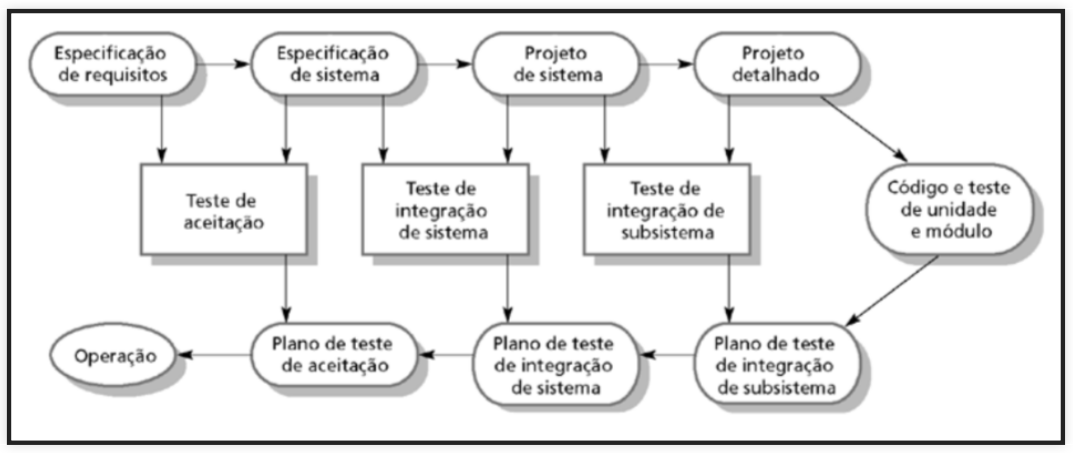
\includegraphics[width=1\hsize]{figuras/fases_de_teste.png}
  %\legend{Texto da legenda quando necessário.}
  \source{\cite{sommerville2013engenharia}}
\end{figure}

Como podemos ver analisando a figura \ref{faseteste} há relacionamento entre as atividades iniciais e finais do processo, isto é, requisitos e decisões de projeto geram os insumos para testes do sistema após sua implementação. Observa-se na figura que, em um primeiro momento, ocorre a `especificação dos requisitos'. Esta, por sua vez, gera com esses requisitos a `especificação do sistema'. Em seguida, ocorre a etapa denominada 'projeto do sistema', que é a criação do sistema num nível macro. O projeto então é detalhado, o que permite a realização da etapa  `codificação e testes de unidade e módulo'. Neste momento iniciam-se as etapas de verificação com o `plano de teste de integração de sistemas' e o `plano de teste de integração de subsistemas'. Nessas duas fases o sistema está sendo integrado, ou seja, primeiro são testadas as partes menores e depois como elas se comunicam. Por último ocorre a validação presente no `plano de teste de aceitação'.

Segundo \citeonline[p.27-28]{sommerville2013engenharia}, existem três processos de teste a serem realizados para obter-se a validação e verificação de um sistema. \textit{Testes de desenvolvimento} são testes realizados em componentes do sistema (entidades simples, classes de objetos etc.). \textit{Testes de sistema} por outro lado, testam o sistema como um todo, focando na iteração entre os componentes do sistema. Por fim, os \textit{testes de aceitação} são testes realizados com dados fornecidos
pelo cliente, que podem identificar erros no sistema ou até mesmo problemas nos requisitos levantados. Os testes de aceitação fazem parte do estágio final do processo de desenvolvimento, e são eles os responsáveis pela validação do sistema. \citeauthoronline{sommerville2013engenharia} afirma também que em uma abordagem incremental cada incremento é testado ao longo de seu desenvolvimento.
Para a figura \ref{faseteste} isso significa que em paralelo são produzidas e realizadas as etapas `teste de aceitação', `teste de integração do sistema', que testa o sistema' como um todo e `teste de integração de subsistema' que testa as partições desse sistema.



Até o presente momento foi falado sobre `verificação' e `validação' sem defini-las. Porém existe uma distinção entre ambas definida pela literatura. Em termos simples, a verificação se preocupa com o funcionamento do sistema de acordo com as técnicas utilizadas. A validação, por outro lado, se refere ao fato de o programa atender os objetivos do implementador, ou seja, atender aos requisitos identificados no início do processo. Isso significa que em algum momento durante o processo de desenvolvimento, o sistema deve ser verificado e validado. 

\begin{figure}[!ht]{10cm}
  \caption{Resumo do processo de desenvolvimento de sistema.} \label{verval}
  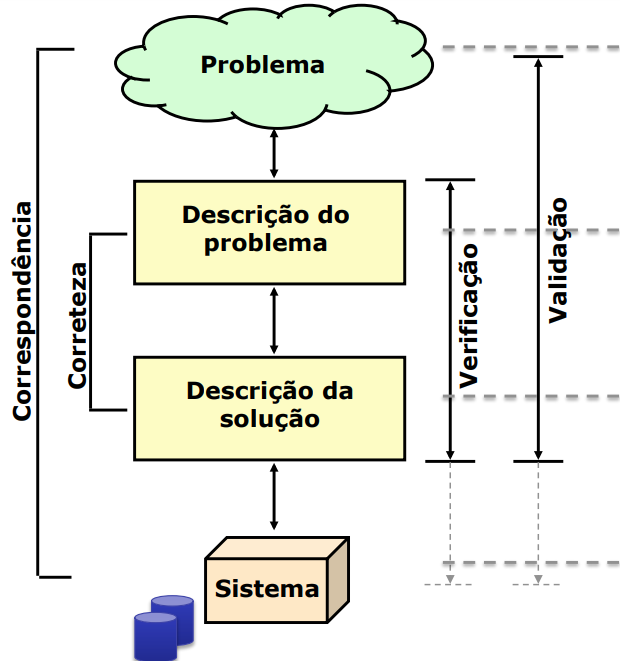
\includegraphics[width=0.5\hsize]{figuras/requisito_proj_proc.png}
  %\legend{Texto da legenda quando necessário.}
  \source{\cite{souza2014banco}}
\end{figure}

A figura \ref{verval} ilustra de forma resumida e simples o assunto descrito nos parágrafos anteriores. Analisando-a entende-se que primeiramente existe um problema a ser trabalhado. O mesmo precisa ser descrito, ou seja, seus requisitos são identificados. A partir dessa descrição é proposta uma solução, que descreve como esses requisitos se comunicam. Assim, da solução proposta se implementa um sistema. O sistema deve atender todas as expectativas levantadas de acordo com o problema identificado para poder ser validado. Já a solução proposta para o problema deve funcionar segundo as técnicas da linguagem utilizada de forma que a solução então possa ser considerada verificada. No capítulo \ref{results} será apresentado como a validação do projeto piloto foi realizada.

Por último, \citeonline{badolato2019b} afirma que deve-se entender que os requisitos podem ser de dois tipos: \textit{requisitos de sistemas} e \textit{requisitos de usuários}.
%definição:
Requisitos de usuários são a descrição, em linguagem natural, em um documento das restrições do sistema com foco no usuário comum, sem grandes conhecimentos computacionais, o cliente.

Requisitos do sistema são requisitos definidos para os subsistemas, que não necessariamente estão descritos segundo os termos do negócio do cliente. Neste caso o documento gerado tem como foco os requisitos implementados do programa ou do banco.

Ao final deste item pode-se concluir que a comunicação entre cliente e equipe de desenvolvimento é essencial para a identificação dos requisitos que permitem o produto final atender as expectativas do cliente, o que implica na validação do produto. A figura \ref{comunicado} exemplifica quando essa comunicação não é eficiente.

\begin{figure}[!ht]{10cm}
  \caption{Ilustração de situação na qual não ocorre uma comunicação eficiente entre cliente e desenvolvedor.} \label{comunicado}
  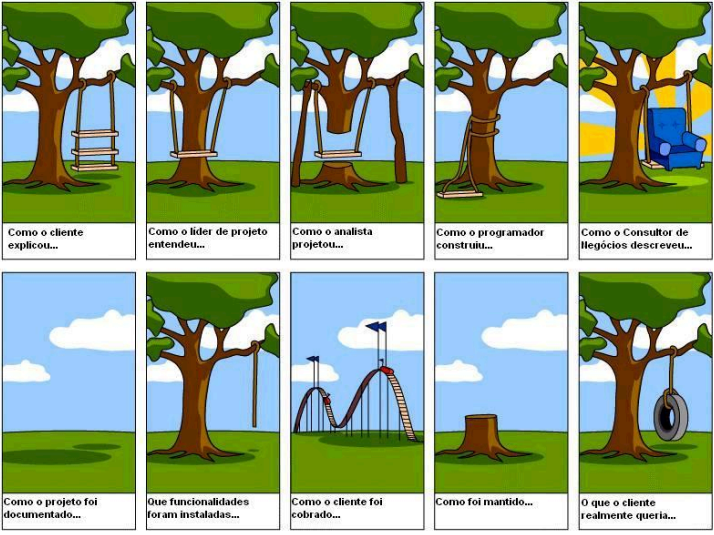
\includegraphics[width=1\hsize]{figuras/requisitos_malcomunicados.png}
  %\legend{Texto da legenda quando necessário.}
  \source{\cite{souza2014banco}}
\end{figure}

\subsection{Linguagens de Modelagem} \label{itemmodl}

\begin{citacao}
``O processo de modelagem conceitual de banco de dados compreende a descrição dos possíveis conteúdos dos dados, além de estruturas e de regras a eles aplicáveis. Essa descrição do banco de dados é feita com base nos construtores semânticos fornecidos por um modelo conceitual'' \cite[p.20]{lisboa2001modelagem}. 
\end{citacao}

Todo modelo trabalha com uma linguagem de modelagem, esta por sua vez ``pode ser composta de pseudo-código, código real, figuras, diagramas ou longas passagens de descrição; na verdade, é praticamente tudo o que ajuda
você a descrever seu sistema. Os elementos que compõem uma linguagem de modelagem são chamados
de notações'' \cite[p.2]{miles2006learning}.

Como apresentado anteriormente no item \ref{sgbdeg}, os tipos de dados a serem armazenados influenciam na escolha tipo de banco de dados, seu modelo e por consequência sua linguagem. Este trabalho tem como foco o acervo de dados do LFSR, constituído principalmente de materiais usados nos projetos de fotogrametria aérea tradicional, o que implica em dados geográficos e seus dados alfanuméricos. Sendo assim, neste item será apresentado algumas das particularidades dos dados geográficos que influenciam na modelagem e as linguagens de modelagem trabalhadas neste trabalho.

\begin{citacao}
    Entende-se por atributo qualquer informação descritiva (nomes, números, tabelas e textos) relacionada com um único objeto, elemento, entidade gráfica ou um conjunto deles, que caracteriza um dado fenômeno geográfico. Nos bancos de dados geográficos, os atributos de objetos geográficos são armazenados em relações convencionais. As representações geométricas destes objetos podem ser armazenadas na mesma tabela que os atributos ou em tabelas separadas, mas ligadas por identificadores únicos.\cite[p.30]{queiroz2006tutorial} 
\end{citacao}
De acordo com \citeonline[p.83-87]{borges2005modelagem}, na modelagem ocorre uma \textit{abstração} de objetos e fenômenos do mundo real assim representando-o, mesmo que de forma simplificada, dentro de um banco de dados. Para os autores a abstração dos conceitos e entidades do mundo real é fundamental na criação de um sistema de informação pois implica na qualidade da tradução dos dados e interações dos objetos desse mundo real para o meio digital. Essa modelagem é demasiada complexa pois envolve a \textit{discretização} do mundo real como parte do processo de abstração, tendo como objetivo uma representação clara dos dados geográficos e seus fenômenos. Existem vários níveis de abstração dos dados geográficos que influenciam no tipo de modelo adotado. São eles:

\begin{itemize}
    \item \textit{Nível do mundo real:} composto pelo objetos geográficos a serem representados. Ex.: rios, estradas, vilas, cidades, vegetação etc.
    \item \textit{Nível conceitual:} usa de um alto nível de abstração. Conceitua formalmente os objetos geográficos a serem modelados determinando as classes contínuas e discretas que entrarão no banco de dados.
    \item \textit{Nível de representação:} neste nível os objetos conceituados do nível conceitual são associadas a classes espaciais, variando de acordo com características como a escala, a projeção ou a visão do usuário. Este nível não possui semelhante no banco de dados tradicional, pois as aplicações tradicionais dificilmente lidam   com a questão da múltipla representação de camadas.
    \item \textit{Nível de implementação:} Define todos os parâmetros necessários para a implementação de forma que respeite os tipos de representações estabelecidos.
\end{itemize}
\begin{figure}[!ht]{10cm}
  \caption{Níveis de especificação de aplicações geográficas.} \label{apli_geo}
  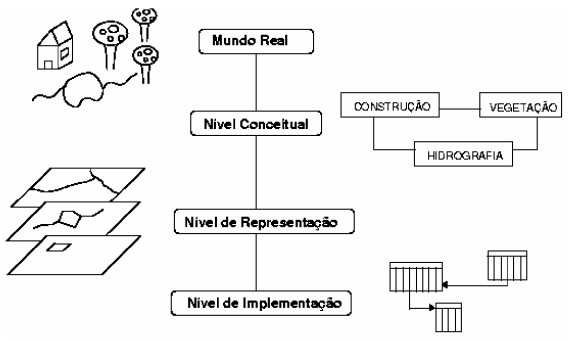
\includegraphics[width=1\hsize]{figuras/apl_geo.png}
  %\legend{Texto da legenda quando necessário.}
  \source{\cite{borges2002modelagem}}
\end{figure}

Corroborando com o explicado acima, \citeonline[p.12-16]{queiroz2006tutorial} afirmam que para a escolha do modelo é necessário se ter uma ideia do conceito de \textit{espaço absoluto} e \textit{espaço relativo}. 

A figura \ref{sao_paulo} exemplifica estes conceitos. Do lado esquerdo aparece um estado onde seus limites geográficos possuem valores de coordenadas correspondentes às estabelecidas na legislação, assim representando o espaço absoluto. Ao lado direito aparece um grafo das conexões entre distritos sobre este mesmo mapa, em forma de rede. No grafo as coordenadas exatas dos distritos não são armazenadas, assim caracterizando essa rede como um modelo de espaço relativo.
No espaço absoluto se encontram os geo-campos e geo-objetos, enquanto o espaço relativo possui o modelo de rede. 

\begin{figure}[!ht]{10cm}
  \caption{Exemplificação de espaço absoluto e espaço relativo.} \label{sao_paulo}
  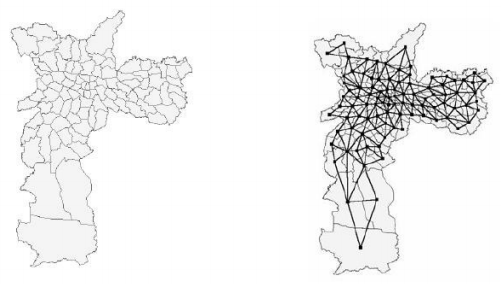
\includegraphics[width=0.75\hsize]{figuras/sao_paulo.png}
  %\legend{Texto da legenda quando necessário.}
  \source{\cite{queiroz2006tutorial}}
\end{figure}


Modelos de geo-campos são normalmente associados aos dados de tipo \textit{raster}. O modelo percebe o espaço geográfico como uma superfície contínua onde observa-se a variação de fenômenos. 
Assim, geo-campos dependem de suas definições físicas no terreno, de forma que se ocorrer uma partição genérica de um geo-campo, o geo-campo resultante possuirá as mesmas propriedades.

Já os modelos de geo-objetos entendem o espaço geográfico como um conjunto de entidades distintas e identificáveis, onde cada entidade possui um fronteira bem definida. Esse modelo normalmente é associado aos dados vetoriais.
Geo-objetos são entidades indivisíveis e singulares, que tem como caraterísticas suas individualidade, fronteiras e atributo. No caso de uma partição genérica, para o conjunto de geo-objetos gerado não estão garantidas as mesmas propriedades que o geo-objeto original.

Já o modelo de rede enxerga o espaço geográfico como um conjunto pontos (entidades), chamados de nós, que se comunicam por linhas, também chamados de arcos. Este modelo é normalmente relacionado a fluxos de transição, linhas de comunicação e acessibilidade etc. Os nós da rede são abstrações das entidades identificadas no terreno, onde as mesmas podem se relacionar de acordo com seus atributos descritivos.

\citeonline[p.21]{lisboa2001modelagem} afirmam que ``um modelo conceitual de dados deve prover construtores especiais para modelar tanto os campos quanto os objetos geográficos. A maioria dos modelos existentes não
suporta a modelagem dos fenômenos geográficos que são percebidos na visão de campo.''

De acordo com \citeonline[p.17] {queiroz2006tutorial} os conceitos apresentados podem ser aglomerados em um conceito genérico chamado de \textit{plano de informação}. Se forem adicionadas as subdivisões de geo-campo: \textit{geo-campo temático}, relacionado a medidas nominais ou racionais, e \textit{geo-campo numérico}, relacionados a medidas de intervalos ou razão, pode-se esquematizar um modelo orientado a objeto que serve como base para dados geográficos. Este esquema é demonstrado na figura \ref{oo_dados_geo}.

\begin{figure}[!ht]{14cm}
  \caption{Modelo orientado a objeto básico para dados geográficos} \label{oo_dados_geo}
  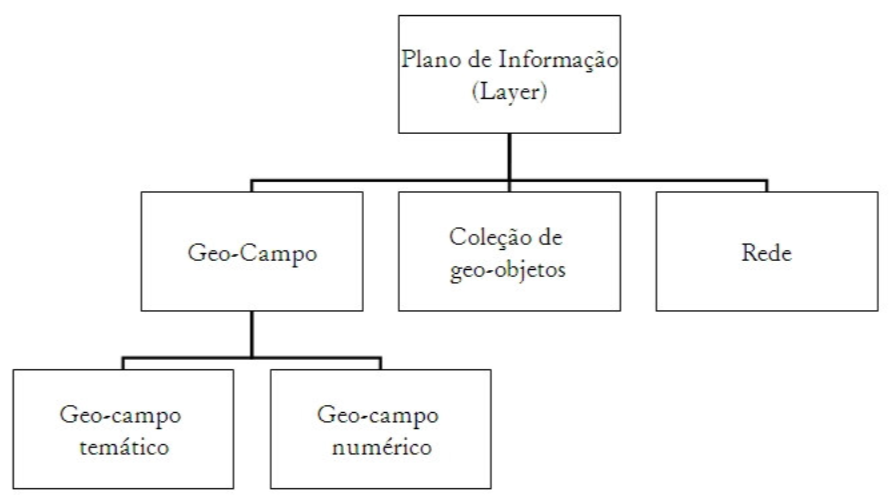
\includegraphics[width=0.75\hsize]{figuras/oo_dados_geo.png}
  %\legend{Texto da legenda quando necessário.}
  \source{\cite{queiroz2006tutorial}}
\end{figure}

Este modelo é facilmente identificado como base para muitos modelos orientados a objetos usados na geo-informação. Como por exemplo os modelos utilizados pelos programas SPRING, ArcGIS, GGIS e TerraLib. 

Segundo \citeonline[p.86]{borges2005modelagem}, existem muitas propostas de extensões para linguagens de modelagem voltadas a aplicações tradicionais de forma a atender as necessidades das aplicações geográficas. São exemplos destas extensões: GeoFrame e OMT-G.

Pode-se definir que
\begin{citacao}
    GeoFrame é um framework conceitual [...], baseado no paradigma de orientação a objetos, para ser usado na modelagem conceitual de bancos de dados geográficos. Este framework utiliza as notações e conceitos da linguagem UML. O objetivo de um framework conceitual é fornecer um conjunto de classes genéricas para um determinado domínio de aplicação para ser usadas como base ou molde para modelar aplicações específicas dentro desse domínio. O produto final de um framework conceitual é um esquema conceitual de dados. \cite[p.43]{queiroz2006tutorial}
\end{citacao}

O modelo OMT-G também é baseado na linguagem UML 
\begin{citacao}
    introduzindo primitivas geográficas com o objetivo de aumentar a capacidade de representação semântica daquele modelo e, portanto reduzindo a distância entre o modelo mental do espaço a ser modelado e o modelo de representação usual. [...] o modelo permite a especificação de atributos alfanuméricos e métodos associados para cada classe. Os principais pontos do modelo são sua expressividade gráfica e sua capacidade de codificação, uma vez que anotações textuais são substituídas pelo desenho de relacionamentos explícitos, que denotam a dinâmica da interação entre os diversos objetos espaciais e não espaciais.\cite[p.88]{borges2005modelagem}
\end{citacao}

Percebe-se que ambos os modelos se baseiam na linguagem UML. Devido à questão de acesso às ferramentas de implementação destes modelos foi decidido trabalhar diretamente com a UML 2.0. Enquanto esta por sua vez não é perfeita para modelagem de dados geográficos, como demonstrado pela existência de extensões propostas do modelo GeoFrame e do modelo OMT-G, estima-se que a linguagem UML 2.0 consegue atender as necessidades de modelagem do banco de dados deste trabalho de forma satisfatória.

\subsubsection{Unified Modeling Language - UML}\label{uml2.0}
\citeonline[p.5-8]{miles2006learning} explica que existe diferenças entre linguagens formais e linguagens informais. A linguagem informal normalmente não possui notações bem definidas. São suscetíveis a ambiguidades, o que leva por sua vez à modelagem equivocada de um conjunto de dados. Outro fator importante é que pela falta de precisão, uma linguagem informal não pode ser codificada. Para evitar esses e outros problemas que se opta por uma linguagem formal.

``A Linguagem de Modelagem Unificada (UML) emergiu como notação diagramática padrão para a modelagem orientada a objetos'' \cite[p.9]{silva2007introuml}. Esta afirmação é corroborada por \citeauthoronline{takai2005intro} quando o mesmo fala que ``o diagrama de classes UML serve geralmente como o esquema para o modelo de dados orientado a objetos'' \cite[p.9]{takai2005intro}.

Segundo \citeonline[p.10-13]{silva2007introuml} e (\citeyear{silva2007classesuml}, p.10-11) a UML 2.0 é composta de 13 diagramas. Definindo diagrama como uma representação gráfica do modelo (parcial ou total). Devido a sua extensa variação de notações, são apresentadas somente as notações pertinentes para o modelo gerado neste trabalho e seus respectivos diagramas. 
Os diagramas de interesse são: 
\begin{itemize}
    \item \textit{Diagrama de Pacotes:} Divide o modelo em `pacotes'. Descrevendo suas iterações em alto nível de abstração. Desta forma, cada pacote vira um sub-sistema composto por partes de um sistema com ao menos um fator em comum.
    \item \textit{Diagrama de Classes:} Considerado o diagrama mais importante da UML, tem como objetivo demonstrar as classes que compõem um sistema, seus atributos e métodos. Demonstrando também como essas classes se relacionam, se complementam e transmitem informações entre si.
    \item \textit{Diagrama de Casos de Uso:} Modela a iteração entre usuário (ator) e o sistema. Determinando o comportamento, as exigências e os resultados que o usuário espera de uma funcionalidade. Desenhado em uma linguagem simples, ilustra o comportamento do sistema.
\end{itemize}

Como toda linguagem formal, a UML 2.0 possui notações específicas. Na figura \ref{uml_obj}, a seguir, algumas dessas notações são apresentadas.

\begin{figure}[!ht]{10cm}
  \caption{Notações da UML A.} \label{uml_obj}
  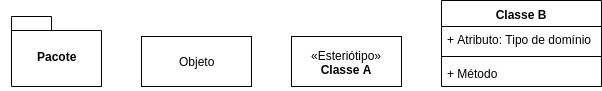
\includegraphics[width=1\hsize]{figuras/uml_obj.png}
  %\legend{Texto da legenda quando necessário.}
  \source{A autora}
\end{figure}

\textbf{Pacote}, em inglês \textit{package} é ``composto por um conjunto de elementos UML que podem ser de qualquer tipo, por exemplo, classes, associações e outras packages'' \cite[p.47]{queiroz2006tutorial}

\citeauthoronline{chonoles2011uml} definem \textbf{objeto} como ``qualquer item útil que tenha identidade, estrutura e comportamento'' \cite[p.46]{chonoles2011uml}, em outras palavras, identifica-se objeto como ``abstração que representa uma entidade do mundo real que pode ser algo concreto [...] ou abstrato'' \cite[p.]{tacla2007analise}.


Para \citeauthoronline{silva2007classesuml} ``\textbf{classe} descreve um conjunto de 
objetos com as mesmas propriedades (\textbf{atributo}), o mesmo comportamento (\textbf{métodos}), os mesmos relacionamentos com outros objetos e a mesma semântica'' \cite[p.11]{silva2007classesuml} corroborado por \citeonline[p.46]{chonoles2011uml} ao afirmar que classe é uma família de objetos. 

Segundo \citeonline[p.11]{silva2007classesuml}, o tipo de dado define o formato em que os dados devem ser armazenados dentro de um atributo, em outras palavras, ``o tipo de dado que descreve os tipos de valores que podem aparecer em cada coluna é presentado por um \textbf{domínio} de valores possíveis'' \cite[p.39]{navathe2011fundamentals}

``Os \textbf{esterótipos} significam um uso ou intenção especial e podem ser aplicados a quase qualquer elemento na notação da UML. Os estereótipos modificam o significado de um elemento e descrevem o papel desses elementos dentro do seu modelo'' \cite[p.16]{miles2006learning}

Como visto na figura \ref{uml_obj}, uma classe pode ser representada com mais de uma divisão, onde a primeira contém seu nome,  segunda seus atributos e a última seus métodos. De acordo com \citeonline[p.12]{silva2007classesuml}, a classe pode aparecer com três, duas ou até somente uma divisão, contudo caso só tenha uma divisão este deve conter as descrições da classe para respeitar as especificações da UML.

\begin{citacao}
    Uma das tarefas mais importantes quando se está modelando os dados de uma aplicação é a identificação de quais os relacionamentos que deverão ser mantidos no banco de dados, dentre os possíveis relacionamentos observáveis na realidade. [...] As cardinalidades associadas aos relacionamentos formam um conjunto de restrições de integridade que devem ser mantidas entre as instâncias dos objetos no banco de dados'' \cite[p.22]{lisboa2001modelagem}.
\end{citacao}

A cardinalidade é representada por uma notação de valores específica desenhada ao lado de fora da junção entre a conexão e uma classe. A tabela \ref{cardinalidade} apresenta alguns desses valores.
\begin{table}[!ht]{14cm}
  \caption{Cardinalidade.}\label{cardinalidade}
    \begin{tabular}{cc}
    \hline
    \rowcolor[HTML]{333333} 
    {\color[HTML]{FFFFFF} \textbf{Multiplicidade}} & {\color[HTML]{FFFFFF} \textbf{Significado}} \\ \hline
    \rowcolor[HTML]{EFEFEF} 
    \begin{tabular}[c]{@{}c@{}}0..1\end{tabular} & \begin{tabular}[c]{@{}c@{}} No mínimo zero (nenhum) e no máximo um. Indica que os objetos\\ das classes associadas não precisam obrigatoriamente estar\\ relacionados, mas se houver relacionamento indica que apenas uma \\ instância da classe se relaciona com as instâncias da outras classe \end{tabular} \\
    \begin{tabular}[c]{@{}c@{}}1..1 \end{tabular} & \begin{tabular}[c]{@{}c@{}} Um e somente um. Indica que apenas um objeto da classe se \\ relaciona com os objetos da outra classe\end{tabular} \\
    \rowcolor[HTML]{EFEFEF} 
    \begin{tabular}[c]{@{}c@{}}0..*\end{tabular} & \begin{tabular}[c]{@{}c@{}}No mínimo nenhum e no máximo muitos. Indica que pode ou não\\ haver instâncias da classe participando do relacionamento \end{tabular} \\
    \begin{tabular}[c]{@{}c@{}}*\end{tabular} & \begin{tabular}[c]{@{}c@{}} Muitos. Indica que muitos objetos da classe estão estão envolvidos\\ no relacionamento\end{tabular} \\
    \rowcolor[HTML]{EFEFEF} 
    \begin{tabular}[c]{@{}c@{}}1..*\end{tabular} & \begin{tabular}[c]{@{}c@{}}No mínimo um e no máximo muitos. Indica que há pelo menos um\\ objeto envolvido no relacionamento, podendo haver muitos\\ envolvidos\end{tabular} \\
    \begin{tabular}[c]{@{}c@{}}3..5\end{tabular} & \begin{tabular}[c]{@{}c@{}}No mínimo três e no máximo cinco. Indica que existem pelo menos\\ três instâncias envolvidas no relacionamento e que podem\\  ser quatro ou cinco as instâncias envolvidas, mas não \\ mais do que isso\end{tabular} \\ \hline
    \end{tabular}
  \source{\cite[p.13]{silva2007classesuml}}
\end{table}

Já os relacionamentos entre classes são desenhados como linhas que conectam essas classes. Cada tipo de relacionamento tem suas particularidades, logo são identificados e desenhados de formas diferentes. A figura \ref{uml_rela} ilustra os relacionamentos da UML e dá suas definições.

\begin{figure}[!ht]{15cm}
  \caption{Notações da UML B.} \label{uml_rela}
  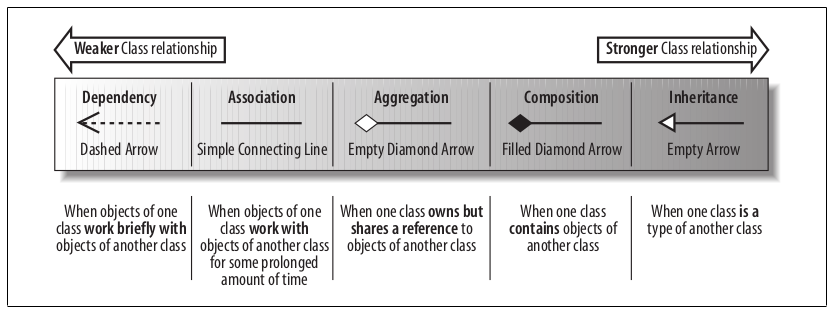
\includegraphics[width=1\hsize]{figuras/uml_relacao.png}
  %\legend{Texto da legenda quando necessário.}
  \source{\cite{miles2006learning}}
\end{figure}

Da figura \ref{uml_rela} tem-se que: `Dependência' ocorre quando objetos de uma classe possuem uma conexão breve com outra classe, `Associação' ocorre quando a conexão entre objetos de duas classes acontece durante um tempo prolongado, `Agregação' ocorre quando uma das classes está contida em outra sem depender da primeira para existir, `Composição' ocorre quando a classe contém objetos de outra classe e `Herança' ocorre quando uma classe é a especialização de outra classe, ou seja, é um tipo da outra classe.

Usando as notações apresentadas lê-se a figura \ref{uml_leitura} da seguinte forma:
a classe B, que é um geometria, agrega classe A, sendo que para cada tupla da classe A existe relacionada ao menos uma tupla da classe B.

\begin{figure}[!ht]{10cm}
  \caption{Ilustração para leitura na UML.} \label{uml_leitura}
  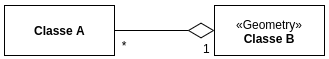
\includegraphics[width=0.75\hsize]{figuras/uml_leitura.png}
  %\legend{Texto da legenda quando necessário.}
  \source{A autora}
\end{figure}

\begin{citacao}
    A coleção de casos de uso representa todos os modos pelos quais o sistema pode ser utilizado pelos atores envolvidos. Um caso de uso é uma sequencia de \textbf{ações} realizadas colaborativamente pelos atores envolvidos e pelo sistema que produz um resultado significativo (com valor) para os atores. Um \textbf{ator} pode ser um usuário ou outro sistema. \cite[p.10]{tacla2007analise}
\end{citacao}


``Especialização de atores representa que um conjunto deles possui responsabilidades ou características em comum '' \cite[p.29]{tacla2007analise}. É importante ressaltar que herança entre atores, generalização e especialização entre atores se refere ao mesmo tipo de relacionamento. Assim, observando a figura \ref{uml_casouso}, identifica-se os atores (a) e (b). O ator (b) é capaz de realizar a ação I, enquanto o ator (a) é capaz de realizar a ação II. Na generalização (c) do ator (b) para o ator (a) tem-se que (b) pode realizar os mesmos casos de uso que (a), o que significa que o ator (b) pode realizar a ação I e a ação II. 

\begin{figure}[!ht]{10cm}
  \caption{Notações da UML C.} \label{uml_casouso}
  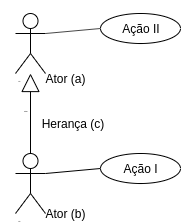
\includegraphics[width=0.5\hsize]{figuras/uml_casosuso.png}
  %\legend{Texto da legenda quando necessário.}
  \source{A autora}
\end{figure}

De acordo com \citeonline[p.10]{tacla2007analise} o diagrama de casos de uso fornece um panorama visual das funcionalidades do sistema, isso significa que uma descrição textual, ou seja um documento de texto é gerado para detalhar os casos de uso.

%falar da relacional(?)
Outra forma de modelar dados, como discutido previamente, é pelo modelo relacional. Enquanto o mesmo não é ideal para modelagem de dados geográficos, como discutido nos últimos itens, devido a uma questão de acessibilidade à ferramenta de implementação em certo momento foi gerado um modelo relacional, logo algumas particularidades não apresentadas até o momento serão descritas a seguir.

\subsubsection{Modelo Entidade-Relacionamento}
``O modelo entidade-relacionamento adota uma
visão natural onde o mundo real consiste em entidades e relacionamentos'' \cite[p.1]{codd1970relational}

\citeauthoronline{heuser1998projeto} afirma que \textbf{entidade} é ``conjunto de objetos da realidade modelada sobre os quais deseja-se manter informações no banco de dados'' \cite[p.23]{heuser1998projeto}, enquanto \textbf{relacionamento} é definido como ``conjunto de associações entre entidades'' \cite[p.24]{heuser1998projeto}. Observando  figura\ref{relacional_a} tem-se que no diagrama 1, A e C são entidades enquanto B é um relacionamento.

\begin{figure}[!ht]{10cm}
  \caption{Ilustração de um diagrama entidade-relacionamento.} \label{relacional_a}
  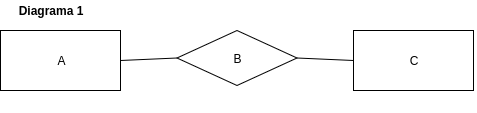
\includegraphics[width=0.75\hsize]{figuras/relacional_a.png}
  %\legend{Texto da legenda quando necessário.}
  \source{A autora}
\end{figure}

Outras duas definições importantes são as de \textbf{chave estrangeira} e \textbf{chave primária}.
\citeonline[p.380]{codd1970relational} define como chave primária (PK - Primary key) uma coluna (ou combinação de colunas) em que seus elementos jamais se repetem. Uma entidade sempre deve possuir ao menos uma PK e a mesma nunca deve ter um elemento nulo. O mesmo autor também define chave estrangeira (FK - Foreign Key) como elementos de uma relação que referenciam outros elementos da mesma relação ou elementos de uma relação diferente. A definição destas chaves é importante viabilizar a integridade de referência, que por sua vez é mecanismo com o qual registramos as relações entre as instâncias do banco de dados.

\begin{figure}[!ht]{10cm}
  \caption{Exemplo de indicação de FK e PK em tabelas.} \label{fk_pk}
  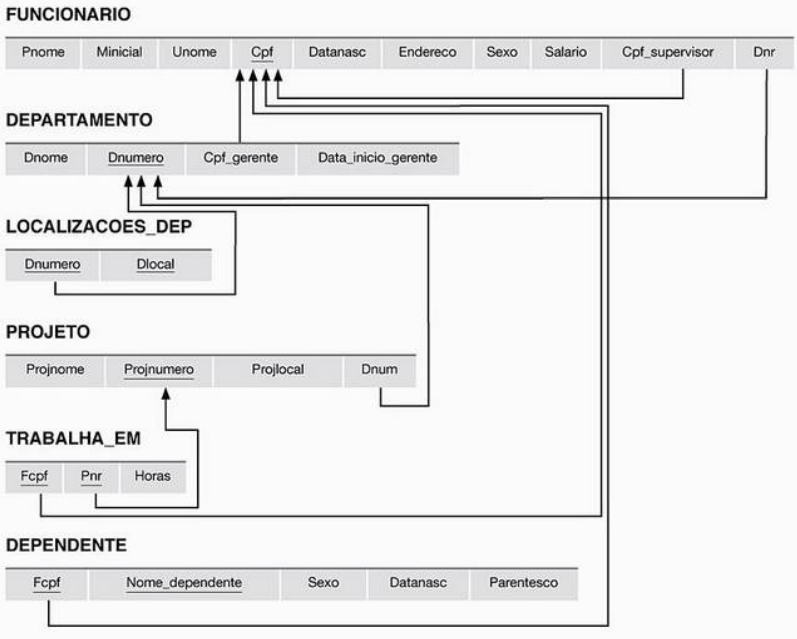
\includegraphics[width=1\hsize]{figuras/fk_pk.png}
  %\legend{Texto da legenda quando necessário.}
  \source{\cite{navathe2011fundamentals}}
\end{figure}
Na figura \ref{fk_pk}, as chaves primárias tem seus nomes sublinhados enquanto as chaves estrangeiras são indicadas pelo uso de `setas', assim o atributo do qual a seta sai se referencia ao atributo à que a seta indica.


\citeonline[p.45-49]{navathe2011fundamentals} usa o termo `relação' para descrever a tabela, logo, relação pode ser tanto entidade quanto relacionamento. Porém um diagrama entidade-relacional pode ser representado de formas diferentes. ``O usuário [...] pode seguir uma disciplina que toda entidade ou relacionamento deve ser mapeado em um registro [...] tudo que você precisa fazer é trocar os diamantes para caixas e para adicionar pontas de seta nas linhas apropriadas'' \cite[p.32]{chen1976entity}. Assim:

\begin{figure}[!ht]{10cm}
  \caption{Ilustração de um diagrama relacional.} \label{relacional_b}
  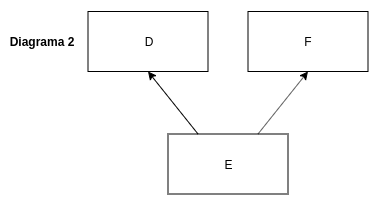
\includegraphics[width=0.5\hsize]{figuras/relacional_b.png}
  %\legend{Texto da legenda quando necessário.}
  \source{A autora}
\end{figure}

No diagrama 2 da figura \ref{relacional_b} sem tem uma dificuldade maior de distinguir relacionamento de entidade porém percebe-se que E possui um chave estrangeira referenciada a D e uma chave estrangeira referenciada a F. É importante mencionar que ``setas no diagrama da estrutura de dados nem sempre representam relações de entidades'' \cite[p.31]{chen1976entity}.

Deve ser lembrado que das linguagens de modelagem apresentadas, somente as partes relevantes para o trabalho foram apresentadas. Suas notações se estendem a mais do que o visto até o presente momento.

\section{Normas}
Existem normas nacionais e internacionais que padronizam como os dados e metadados de tipos específicos devem ser modelados e implementados. Durante a construção do projeto piloto, visando a padronização apresentada nesses documentos, foi realizada uma pesquisa sobre normas, tanto nacionais quanto internacionais, que pudessem ser utilizadas neste trabalho. 

Dentre as normas nacionais existe o \textit{Perfil de Metadados Geoespaciais do Brasil - PMGB}. 
Segundo \citeonline[p.86]{inde2010} devido à tendência mundial na época da definição de perfis de metadados geográficos baseados na ISO:19115:2003, a CONCAR (Comissão Nacional de Cartografia) especificou e consolidou o PMGB através do CEMG (Comitê de Estruturação de Metadados Geoespaciais). ``Trata-se de uma iniciativa para ordenar a geração, armazenamento, acesso, compartilhamento, divulgação e uso dos dados geoespaciais - aqueles que se distinguem pela componente espacial, que associa cada entidade ou fenômeno a uma localização na Terra '' \cite[p.10]{pmgb2009}

``A proposta do Perfil MGB inclui a maioria das seções de metadados presentes na norma ISO 19115'' \citeonline[p.86]{inde2010}. Dentre eles os mais relevantes para o trabalho são \textbf{MD\_SpatialRepresantation}, relativos as informações de representação espacial e \textbf{MD\_ReferenceSystem}, responsável por descrever o sistema de referencia utilizado.  

Já no âmbito internacional, para dados geoespaciais, a organização de padronização mais importante é o \textit{Open Geospacial Consortium - OGC}. 
\begin{citacao}
O Open Geospatial Consortium (OGC) é um consórcio internacional de mais de 530 empresas, agências governamentais, organizações de pesquisa e universidades orientadas a tornar informações e serviços geoespaciais (localização) FAIR -Findable, Accessible, Interoperable, and Reusable (Localizáveis, Acessíveis, Interoperáveis e Reutilizáveis). \cite[p.1]{ogc}
\end{citacao}

``Os produto do trabalho do OGC são apresentados sob forma de especificações de interfaces e padrões de intercâmbio de dados'' \cite[p.66]{queiroz2006tutorial}.

Porém tanto o PMGB, quanto a documentação da OGC baseia-se nos documentos produzidos pela \textit{International Organization for Standardization - ISO's}.

\begin{citacao}
    A ISO é uma organização internacional não governamental independente, com 164 membros de organismos nacionais de padrões. Por meio de seus membros, reúne especialistas para compartilhar conhecimento e desenvolver Normas Internacionais voluntárias, baseadas em consenso e relevantes para o mercado, que apoiam a inovação e fornecem soluções para os desafios globais. [...] A ISO publicou 22873 Normas Internacionais e documentos relacionados, cobrindo quase todos os setores, desde tecnologia, segurança alimentar, agricultura e saúde.\cite[p.1]{iso}
\end{citacao}


A ISO / TC 211 é um comitê técnico, responsável pela elaboração de ISO's relacionadas as informações geográficas digitais. Seu trabalho esta intimamente ligado à produção da documentação gerada pela OGC.

Dentre as ISO's elaboradas pela ISO/TC 211  disponíveis, algumas das que foram pesquisadas, de acordo com \citeauthoronline{isomodels}, são:
\begin{itemize}
    \item ISO 6709 Standard representation of geographic point location by coordinates - Trata da representação de latitude, longitude e altitude de pontos geográficos.
    \item ISO 19115 Metadata - Trata de metadados relacionados direta ou indiretamente a dados geográficos.
    \item ISO 19123 Schema for coverage geometry and functions - Define um modelo abstrato de coberturas geográficas.
    \item ISO 19129 Imagery, gridded and coverage data - Gera uma estrutura aplicada para software que tratam de dados relacionados ao sensoriamento remoto, a fotogrametria e ao processamento de imagem, como imagens, coberturas etc.
    \item ISO 19130 Imagery sensor models for geopositioning - Trata de dados e metadados de sensores com o objetivo de fornecer uma interoperabilidade para dados de imagens.
    \item ISO 19136 Geography Markup Language (GML) - Trata da codificação do xml voltado para informações geográficas.
    \item ISO 19159 Calibration and validation of remote sensing imagery sensors and data - Trata dos padrões necessários para a validação e calibração de sensores imageadores aéreos e orbitais.
\end{itemize}

A partir dessa pesquisa percebeu-se uma ausência de normas nacionais voltadas exclusivamente para os dados fotogramétricos. Durante a mesma ocorreu uma dificuldade no acesso aos documentos por inteiro das ISO's, acarretando no acesso limitado aos dados públicos ou parciais desses documentos. Deste acesso percebeu-se não haver uma ISO que trata-se exclusivamente de dados voltados para a fotogrametria. Baseado nessas experiências julgou-se não haver normas estabelecidas e acessíveis, tanto em âmbito nacional quanto internacional, que atendessem às necessidades deste trabalho. Assim, foi decidido pela modelagem independente dos dados fotogramétricos, como demonstrado na metodologia apresentada no capítulo \ref{met}, tomando por base principalmente os modelos pré-existentes de trabalhos anteriores no projeto E-foto. 

